\documentclass[draft]{Report/thuemp}
\begin{document}

% 标题,作者
\emptitle{光学信息处理与傅里叶光学}
\empauthor{王驰}{王合英}

% 奇数页页眉 % 请在这里写出第一作者以及论文题目
\fancyhead[CO]{{\footnotesize 王驰: 光学信息处理与傅里叶光学}}

%%%%%%%%%%%%%%%%%%%%%%%%%%%%%%%%%%%%%%%%%%%%%%%%%%%%%%%%%%%%%%%%
% 关键词 摘要 首页脚注
%%%%%%%%关键词
\Keyword{光学信息处理,傅里叶光学,空间滤波,阿贝成像,衍射,卷积定理}
\twocolumn[
\begin{@twocolumnfalse}
\maketitle

%%%%%%%%摘要
\begin{empAbstract}
本实验利用基于 4F 结构的光学系统,系统研究了傅里叶光学的基本原理及其在信息处理中的应用。通过观察一维光栅($12\ \mathrm{line/mm}$)和二维正交光栅(“光”字屏)的夫琅禾费衍射图样,直观验证了会聚透镜的傅里叶变换性质,频谱面上的空间频率分布与物函数的周期和方向严格对应;利用自制滤波器(小孔、挡板、狭缝)实现了空间滤波,包括低通(图像模糊)、高通(边缘增强)及方向滤波(特定纹理提取);通过复合光栅滤波器($f_1=100\ \mathrm{line/mm}$, $f_2=102\ \mathrm{line/mm}$)观察到光学微分效应,突出了图像边缘;实验还通过两个卷积件的复合衍射,在频域验证了卷积定理;最后,利用 $\theta$ 调制片和白光光源实现了假彩色编码。实验结果直观地展示了在空间频域中处理信息的有效性,为光学计算和现代成像技术提供了实验基础。
\end{empAbstract}

%%%%%%%%英文标题、作者、摘要、关键词
\emptitleEn{Experiments of Modern Physics in Tsinghua University}
\empauthorEn{Chi Wang}{Heying Wang}
\KeywordEn{Optical Information Processing, Fourier Optics, Spatial Filtering, Abbe Imaging, Diffraction, Convolution Theorem}

\begin{empAbstractEn}
This experiment systematically investigated the fundamental principles of Fourier optics and its applications in information processing using a 4F-based optical system. The Fourier transform property of converging lenses was verified by observing the Fraunhofer diffraction patterns of a 1D grating ($12\ \mathrm{line/mm}$) and a 2D orthogonal grating ("Guang" character), showing strict correspondence between spatial frequency distribution and object properties. Spatial filtering, including low-pass (blurring), high-pass (edge enhancement), and directional filtering (texture extraction), was implemented using custom-made filters (pinholes, stops, slits). The optical differentiation effect, which enhances image edges, was observed using a composite grating filter ($f_1=100\ \mathrm{line/mm}$, $f_2=102\ \mathrm{line/mm}$). The convolution theorem was also experimentally verified in the frequency domain using composite diffraction elements. Finally, pseudo-color encoding was achieved through $\theta$ modulation using a white light source. The results vividly demonstrate the efficacy of processing information in the spatial frequency domain, providing an experimental foundation for optical computing and modern imaging technologies.
\end{empAbstractEn}

%%%%%%%%首页角注,依次为实验时间、报告时间、学号、email
\empfirstfoot{2025-05-18}{2025-05-25}{2022012259}{chi-wang22@mails.tsinghua.edu.cn}
\end{@twocolumnfalse}
]
%%%%%%%%!首页角注可能与正文重叠,请通过调整正文中第一页的\enlargethispage{-3.3cm}位置手动校准正文底部位置:
%%%%%%%%%%%%%%%%%%%%%%%%%%%%%%%%%%%%%%%%%%%%%%%%%%%%%%%%%%%%%%%%
%  正文由此开始
\wuhao 
%  分栏开始

\section{实验仪器}
\enlargethispage{-3.3cm}

本实验使用氦氖激光器( $\lambda=632.8\ \mathrm{nm}$ )作为相干光源,搭建如图 \ref{fig:setup} 所示的空间滤波实验光路。激光束经 $\mathrm{L_1}$ 扩束、$\mathrm{L_2}$ 准直后形成平行光,照射位于物面上的透明物体。$\mathrm{L_3}$ 为傅里叶变换透镜(焦距 $F=16.0\ \mathrm{cm}$ ),其后焦面 F 即为频谱面,用于放置各种滤波器。像面位于与物面关于 $L_3$ 共轭的位置,此处放置一电荷耦合装置(Charge Coupled Device, CCD)用于观察和记录滤波后的图像。这一组装置被用于空间成分滤波实验和方向滤波实验。

在 $\mathrm{L_3}$ 后方距离 $2F = 320 \ \mathrm{cm}$ 处,补充放置一焦距同为$F$的透镜 $\mathrm{L_4} $,并选择 $\mathrm{L_4}$ 后方距离$F$处作为像面,由此构成一个 $4F$ 系统。这一组装置被用于完成验证卷积定理、光学微分,以及$\theta$调制实验。

在以上实验装置中,透镜 $\mathrm{L_3}$ 均为在光学上实现光场傅里叶变换的核心器件。在薄透镜近似下,透镜作用相当于为从不同位置透过透镜的光添加一个额外相位$\Delta \varphi$。取图【】所示坐标系,考察一束平行光入射后会聚到焦点上的情形。根据费马(Fermat)原理,可以写出

\begin{align}
    \Delta \varphi (\xi, \eta) + k \sqrt{\xi^2+\eta^2+F^2} = \text{Const.}
\end{align}

傍轴近似下($x, x', y, y' \ll F $),定取相位基准$\Delta \varphi (\xi=0, \eta=0) = 0$,可以近似写出:

\begin{align}
    \Delta \varphi (\xi, \eta) = -k \frac{\xi^2+\eta^2}{2F}
\end{align}

现在考虑物面上的光场分布 $g(x,y)$ 与 $\mathrm{L_3}$ 的后焦面上光场分布 $G(x', y')$ 的关系:利用惠更斯(Huygens)原理,考察通过透镜后的子波叠加,可以写出:

\begin{align}
            &   % Split 01
            G(x', y')
        \notag \\
            \propto
            &   % Split 01   
            \iint
            \mathrm{d}x \mathrm{d}y \ g(x,y)
            \times \exp \Bigl\{
                -i \Delta \varphi(\xi, \eta)
            \Bigr.
        \notag \\
            &
            \quad
                - ik \sqrt{(x-\xi)^2+(y-\eta)^2+F^2}
        \notag \\
            &   % Split 01
            \quad \Bigl.
                - ik \sqrt{(x'-\xi)^2+(y'-\eta)^2+F^2}
            \Bigr\}
\end{align}

傍轴近似下($x, x', y, y' \ll F $),假定透镜尺寸足够大,以至于光阑半径的效应可以忽略($R \gg \sqrt{\lambda F}$,$R$表示透镜特征尺度,下同),同时又不太大,不致破坏傍轴近似条件($R \ll F$);展开各平方根项并忽略高阶项,可以得到:

\begin{align}
        &
        G(x', y')
    \notag \\
        \propto
        &
        \iint \mathrm{d}x \mathrm{d}y \mathrm{d}\xi \mathrm{d}\eta \, g(x,y)
    \notag \\
        & 
        \times \exp \Bigl\{
            -   ik \frac{ (x - \xi) ^ 2 + (y - \eta) ^ 2 }{2F}
            +   ik \frac{ \xi ^ 2 + \eta ^ 2 }{2F}
        \Bigr.
    \notag \\
        &
        \quad \quad \Bigl.
            -   ik \frac{ (x' - \xi) ^ 2 + (y' - \eta) ^ 2}{2F}
            -   2ikF
        \Bigr\}
    \notag \\
        =
        &
        \exp\bigl(-2ikF\bigr)
        \iint \mathrm{d}x \mathrm{d}y \mathrm{d}\xi \mathrm{d}\eta \, g(x,y)
    \notag \\
        &
        \times \exp \Bigl\{
            -   ik \frac{x^2+y^2+x'^2+y'^2+\xi^2+\eta^2}{2F}
        \Bigr.
    \notag \\
        &
        \quad \quad \Bigl.
            +   ik \frac{(x+x')\xi + (y+y')\eta}{F}
        \Bigr\}
    \notag \\
        =
        &
        \exp\bigl(-2ikF\bigr)
        \iint \mathrm{d}x \mathrm{d}y \mathrm{d}\xi \mathrm{d}\eta \, g(x,y)
    \notag \\
        &
        \times \exp \Bigl\{
            +   ik \frac{xx'+yy'}{2F}
        \Bigr.
    \notag \\
        &
        \quad \quad \Bigl.
            -   ik \frac{
                \bigl[\xi  - (x+x')\bigr]^2
            +   \bigl[\eta - (y+y')\bigr]^2
            }{2F}
        \Bigr\}
    \notag \\
        =
        &
        \exp\bigl(-2ikF\bigr)
        \iint \mathrm{d}x \mathrm{d}y  \, g(x,y) \exp \Bigl\{
            +   ik \frac{xx'+yy'}{2F}
        \Bigr\}
    \notag \\
        &
        \times \int_{-\infty}^{+\infty} \mathrm{d}\xi \exp \Bigl\{
            -   ik \frac{
                \bigl[\xi  - (x+x')\bigr]^2
            }{2F}
        \Bigr\}
    \notag \\
        &
        \times \int_{-\infty}^{+\infty} \mathrm{d}\eta \exp \Bigl\{
            -   ik \frac{
                \bigl[\eta - (y+y')\bigr]^2
            }{2F}
        \Bigr\}
    \notag \\
        \propto
        &
        \iint \mathrm{d}x \mathrm{d}y \, g(x,y) \exp \Bigl\{
            +   ik \frac{xx'+yy'}{2F}
        \Bigr\}
\end{align}

这就表明,在透镜 $\mathrm{L_3}$ 的后焦面上,光场分布 $G(x', y')$ 与物面光场分布 $g(x,y)$ 之间满足傅里叶变换关系:

\begin{align}
    G(x', y') \propto \mathcal{F}\bigl\{g(x,y)\bigr\} \Bigl(f_x = \frac{x'}{\lambda F}, f_y = \frac{y'}{\lambda F}\Bigr)
\end{align}

其中参数$f_x, f_y$分别为物面光场沿$x$和$y$方向的空间频率,而通过$f_x = \frac{x'}{\lambda F}, f_y = \frac{y'}{\lambda F}$的关系式与透镜 $\mathrm{L_3}$ 的后焦面上的空间点联系,$\mathrm{L_3}$ 的后焦面因而被称为为空间频谱面。

以上述傅里叶变换关系为基础,开展以下各项实验。

\section{实验内容}
 

\subsection{空间成分滤波}
使用一维光栅($10\ \textrm{线/mm}$),条纹沿竖直方向放置,构建物面光场。在频谱面 $F$ 处预期可观察到水平排列的衍射图样,也即物面光场的空间频率分布。

使用硬纸打孔,按下列情况分别允许特定空间频率成分通过,在像面借助CCD观察并记录条纹间距和形貌的变化,进行比较:

\begin{itemize}
    \item A组:分别通过 (0, $\pm 1$ 级)、(0, $\pm 2$ 级),以及不加滤波器;
    \item B组:分别通过 (0, +1 级)、(0, $\pm 1$, $\pm 2$ 级),以及不加滤波器;
    \item C组:分别通过 (仅 0 级)、(除 0 级外所有),以及不加滤波器。
\end{itemize}

其中,A组和B组用于分析不同频率成分对图像周期和形貌的影响,C组用于分析零频分量对图像的影响。

\subsection{方向滤波}
在物面放置正交光栅(“光”字屏),观察其二维点阵频谱。同样利用硬纸开孔,分别只允许以下方向的频谱分量通过:

\begin{itemize}
    \item 竖直方向(即只通过频谱的水平分量);
    \item 水平方向(即只通过频谱的竖直分量);
    \item $\pm 45^\circ$ 斜方向。
\end{itemize}

继续在像面借助CCD观察并记录像面图像的变化,分析频谱方向与图像特征方向的关系;进而使用图像分析软件,测量水平条纹与$45^\circ$斜方向条纹的空间周期之比。

\subsection{验证卷积定理}

傅里叶变换的重要性质之一为卷积定理。对于函数 $g_1(x,y)$ 和 $g_2(x,y)$,其卷积定义为:

\begin{align}
        \bigl(g_1 \ast g_2\bigr) & (x,y) % Very special alignment here.
    \notag \\
        =
        &
        \iint \mathrm{d}x' \mathrm{d}y' \ g_1(x', y') g_2(x-x', y-y')
\end{align}

卷积定理指出,函数的卷积在频域中对应于各自傅里叶变换的乘积:

\begin{align}
    \mathcal{F}\bigl\{g_1 \ast g_2\bigr\} = \mathcal{F}\bigl\{g_1\bigr\} \cdot \mathcal{F}\bigl\{g_2\bigr\}
\end{align}

使用图【】所示的 $4F$ 系统,在频谱面上单独放置透明卷积件时,其振幅透光率函数 $G_i(\xi,\eta) \quad (i = 1, 2) $ 的傅里叶变换即为物面光场 $g_i(x,y)$。若将两个卷积件依次密接放置在频谱面上,可观察像面图像 $g(x,y)$,验证其是否等于各自物面光场的卷积,进而达到验证卷积定理的目的。

考虑到卷积运算的难度,本部分实验中选择两块二维光栅作为卷积件,以简化验证过程;通过分别转动两块光栅,实现对两个原函数 $g_1(x,y)$ 和 $g_2(x,y)$ 的改变,以更充分地验证卷积定理。

根据上述理论预测,在像面上观测到的衍射图样应是,以其中一块卷积件形成的点阵图样为基本单元,根据另一块卷积件的空间周期和方向进行重复排列所形成的图样。

\subsection{光学微分}

对于正弦光栅,其振幅透光率写成$ H(\xi, \eta) = H_0 + H_1\cos (2\pi f_0 \xi + \varphi_0)$ ,其傅里叶变换为:

\begin{align}
        h_0 & (x', y') % Very special alignment here.
    \notag \\
        =
        &
        H_0 \delta(x', y') + \frac{H_1}{2} \Bigl[
            \delta\Bigl(x' - \frac{f_0}{\lambda F}, y'\Bigr) e^{i\varphi_0}
        \Bigr.
    \notag \\
        &
        \Bigl.
        +   \delta\Bigl(x' + \frac{f_0}{\lambda F}, y'\Bigr) e^{-i\varphi_0}
        \Bigr]
\end{align}

引入复合光栅,其振幅透光率中包含两个频率成分:
\begin{align}
        H(\xi, \eta) 
        &
        H_0 + H_1\cos (2\pi f_1 \xi + \varphi_1)
        \notag \\
        &
        + H_2\cos (2\pi f_2 \xi + \varphi_2)
\end{align}

则其傅里叶变换为:
\begin{align}
        h & (x', y')
    \notag \\
        =
        &
        H_0 \delta(x', y') + \frac{H_1}{2} \Bigl[
            \delta\Bigl(x' - \frac{f_1}{\lambda F}, y'\Bigr) e^{i\varphi_1}
        \Bigr.
    \notag \\
        &
        \Bigl.
        +   \delta\Bigl(x' + \frac{f_1}{\lambda F}, y'\Bigr) e^{-i\varphi_1}
        \Bigr]
        + \frac{H_2}{2} \Bigl[
            \delta\Bigl(x' - \frac{f_2}{\lambda F}, y'\Bigr) e^{i\varphi_2}
        \Bigr.
    \notag \\
        &
        \Bigl.
        +   \delta\Bigl(x' + \frac{f_2}{\lambda F}, y'\Bigr) e^{-i\varphi_2}
    \Bigr]
\end{align}

考察复合光栅的两个频率成分各自给出的$+1$级像(以$x' = \frac{f_{1,2}}{\lambda F}$为中心);借助卷积定理得到,对应的像面光场为:
\begin{align}
        g_{+1} & (x', y')
    \notag \\
        =
        &
        \frac{H_1}{2} g\Bigl(x' - \frac{f_1}{\lambda F}, y'\Bigr) e^{i\varphi_1} +
        \frac{H_2}{2} g\Bigl(x' - \frac{f_2}{\lambda F}, y'\Bigr) e^{i\varphi_2}
\end{align} 

考察以下情形:$f_2 = f_1 + \Delta f, \Delta f \ll f_1$,并且$H_1=H_2, \varphi_1 - \varphi_2 = (2k+1)\pi \quad (k\in \mathbb{Z})$则可以对上述式子进行泰勒展开,得到:
\begin{align}
        & g_{+1} (x', y')
    \notag \\
        =
        &
        \frac{H_1}{2} \Bigl[
            g\Bigl(x' - \frac{f_1}{\lambda F}, y'\Bigr) -
            g\Bigl(x' - \frac{f_1 + \Delta f}{\lambda F}, y'\Bigr)
        \Bigr] e^{i\varphi_1}
    \notag \\
        \approx
        &
        - \frac{H_1 \Delta f}{2 \lambda F} e^{i\varphi_1} \times \frac{\partial g}{\partial x'} \Bigl(x' - \frac{f_1}{\lambda F}, y'\Bigr)
\end{align}

这表明,在上述条件下,复合光栅的$+1$级像近似为物面图像在$x$方向的微分。同理可得$-1$级像也具有类似的微分特性。

本实验中,在物面放置以图片(形状如图【】所示),在频谱面 F 处放置复合正弦光栅($f_1=100\ \textrm{线/mm}$, $f_2=102\ \textrm{线/mm}$)作为空间滤波器,在像面 $\pm 1$ 级衍射像处,预期可观察到图像的微分效果。垂直于光轴缓慢平移复合光栅,寻找并记录使 $\pm 1$ 级像的边缘轮廓最清晰的位置,拍摄记录。

\subsection{\texorpdfstring{$\theta$}{theta} 调制}
$\theta$片由多块不同取向的一维光栅拼成。使用白光入射,频谱面上依各个光栅取向形成一系列不同颜色的衍射光斑阵列。在频谱面上叠加孔阵滤波器,在适当的方向上保留适当颜色的$\pm 1$级衍射斑。在像面上,将能够得到一幅彩色图像。

本实验中,$\theta$片为一块三个取向光栅拼成的风景图样,三个光栅取向两两互成 $60^\circ$ 角,空间频率均为 $100\ \textrm{线/mm}$。同样使用硬纸打孔制作滤波器,在频谱面上仅允许三个方向的 $\pm 1$ 级衍射斑通过,在像面上观察并记录彩色图像。

\section{实验结果与分析}

\subsection{空间成分滤波}

% A组对比分析

\begin{figure*}[htbp]
    \centering
    \begin{subfigure}[b]{0.3\textwidth}
        \centering
        \includegraphics[width=0.9\textwidth]{Data/001/10_per_mm-baseline.png}
        \subcaption{不加滤波器}
        \label{fig:spatial_filter_a_base}
    \end{subfigure}
    \hfill
    \begin{subfigure}[b]{0.3\textwidth}
        \centering
        \includegraphics[width=0.9\textwidth]{Data/001/10_per_mm-0_pm1_only.png}
        \subcaption{仅允许(0, $\pm 1$ 级)通过}
        \label{fig:spatial_filter_a_pm1}
    \end{subfigure}
    \hfill
    \begin{subfigure}[b]{0.3\textwidth}
        \centering
        \includegraphics[width=0.9\textwidth]{Data/001/10_per_mm-0_pm2_only.png}
        \subcaption{仅允许(0, $\pm 2$ 级)通过}
        \label{fig:spatial_filter_a_pm2}
    \end{subfigure}
    \captionnamefont{\wuhao\bf\heiti}
    \captiontitlefont{\wuhao\bf\heiti}
    \caption{空间成分滤波实验结果A组对比图}
    \label{fig:spatial_filter_a}
\end{figure*}

空间成分滤波A组对比如图\ref{fig:spatial_filter_a}所示。相比较于不放滤波器情形,可以观察到:仅保留$0, \pm 1 $级频率成分所得到的图像中,衍射条纹周期与不放置滤波器时相当,而条纹的明暗交界处则变得较为模糊;仅保留$0, \pm 2$级频率成分所得到的图像中,衍射条纹周期减小至不放置滤波器时的大约一半,并同样出现条纹明暗交界处变模糊的现象。

通过A组对比可以看出:保留不同级次的衍射光,会直接影响像面条纹的周期和清晰度。当仅保留 $0, \pm 1$ 级时,图像保持了与原光栅相同的空间周期($d \approx 1/f_0$),因为 $\pm 1$ 级衍射对应于光栅的基频;而当仅保留 $0, \pm 2$ 级时,像面条纹周期减半($d' \approx 1/(2f_0)$),这是因为 $\pm 2$ 级对应的是二倍频率成分。两种情况下条纹边缘均较为模糊,提示单一频率成分不足以完整重建物体的细节结构。这一点将在接下来的B组对比中得到进一步说明。

% B组对比分析

\begin{figure*}[htbp]
    \centering
    \begin{subfigure}[b]{0.3\textwidth}
        \centering
        \includegraphics[width=0.9\textwidth]{Data/001/10_per_mm-baseline.png}
        \subcaption{不加滤波器}
        \label{fig:spatial_filter_b_base}
    \end{subfigure}
    \hfill
    \begin{subfigure}[b]{0.3\textwidth}
        \centering
        \includegraphics[width=0.9\textwidth]{Data/001/10_per_mm-0_pm1_only.png}
        \subcaption{仅允许(0, $\pm 1$ 级)通过}
        \label{fig:spatial_filter_b_pm1}
    \end{subfigure}
    \hfill
    \begin{subfigure}[b]{0.3\textwidth}
        \centering
        \includegraphics[width=0.9\textwidth]{Data/001/10_per_mm-0_pm2_only.png}
        \subcaption{仅允许(0, $\pm 1$, $\pm 2$ 级)通过}
        \label{fig:spatial_filter_b_pm1_pm2}
    \end{subfigure}
    \captionnamefont{\wuhao\bf\heiti}
    \captiontitlefont{\wuhao\bf\heiti}
    \caption{空间成分滤波实验结果B组对比图}
    \label{fig:spatial_filter_b}
\end{figure*}

空间成分滤波B组对比如图\ref{fig:spatial_filter_b}所示。相比较于不放滤波器情形,仅保留$0, \pm 1$级,以及仅保留$0, \pm 1, \pm 2$级的情形,衍射条纹的间距均未发生显著改变,而条纹的明暗交界处仍然以不放滤波器最为清晰,仅保留$0, \pm 1$级的情形中,条纹的明暗交界处则变得最为模糊,仅保留$0, \pm 1, \pm 2$级的情形中,条纹的明暗交界清晰程度则介于两者之间。

通过B组对比可以看出,增加更多的频率成分可以提升图像的清晰度和保真度。保留的频率成分越多,图像的边缘越锐利,越接近原始物体的形貌。这是因为高频成分主要贡献了图像的边缘和细节信息,而低频成分则主要贡献了图像的整体轮廓和大尺度结构。

% C组对比分析

\begin{figure*}[htbp]
    \centering
    \begin{subfigure}[b]{0.3\textwidth}
        \centering
        \includegraphics[width=0.9\textwidth]{Data/001/10_per_mm-baseline.png}
        \subcaption{不加滤波器}
        \label{fig:spatial_filter_c_base}
    \end{subfigure}
    \hfill
    \begin{subfigure}[b]{0.3\textwidth}
        \centering
        \includegraphics[width=0.9\textwidth]{Data/001/10_per_mm-0_only.png}
        \subcaption{仅允许 0 级通过}
        \label{fig:spatial_filter_c_0}
    \end{subfigure}
    \hfill
    \begin{subfigure}[b]{0.3\textwidth}
        \centering
        \includegraphics[width=0.9\textwidth]{Data/001/10_per_mm-0_excluded.png}
        \subcaption{滤除 0 级(所有其他级通过)}
        \label{fig:spatial_filter_c_no0}
    \end{subfigure}
    \captionnamefont{\wuhao\bf\heiti}
    \captiontitlefont{\wuhao\bf\heiti}
    \caption{空间成分滤波实验结果C组对比图}
    \label{fig:spatial_filter_c}
\end{figure*}

空间成分滤波C组对比如图\ref{fig:spatial_filter_c}所示。仅保留 0 级频率成分时,像面呈呈现亮背景,完全看不到原先在$x$轴方向表现出的周期性条纹结构,而仅能见到若干杂散的干涉条纹;而滤除 0 级、保留所有其他高频成分时,像面仍可观察到清晰的条纹结构,但条纹整体亮度以及对比度显著降低。

这一结果表明:0 级频率成分(零频分量)对应于物体的平均透光率,决定了图像的整体亮度和背景;而高阶频率成分则携带了物体的周期性结构和细节信息。去除零频分量相当于实现了高通滤波,可以突出图像的边缘和快速变化的细节,但会损失直流背景信息。

综合A、B、C三组实验结果可以看出:图像的周期性特征由最低阶非零频率成分($\pm 1$ 级)决定;图像的清晰度和细节则需要更多的高频成分来重建;零频分量则决定了图像的整体亮度。这充分验证了傅里叶光学中物面图像与频谱面空间频率分布之间的对应关系,也直观展示了空间滤波在图像处理中的作用机制。

\subsection{方向滤波}

\begin{figure*}[htbp]
    \centering % 全局居中,让每一行都在页面中间
    
    % --- 设置参数 ---
    % 定义子图宽度 (例如 0.3\textwidth,保证 3张图 + 间距 < 1.0\textwidth)
    % 0.3 * 3 = 0.9,剩下 10% 空间留给间距和边距
    
    % --- 第一排:3张图 ---
    \begin{subfigure}[b]{0.3\textwidth}
        \centering
        \includegraphics[width=0.9\textwidth]{Data/002/2dim_baseline_02.png}
        \subcaption{不加滤波器}
        \label{fig:directional_filter_baseline}
    \end{subfigure}% 
    \hspace{0.03\textwidth}% --- 固定的水平间距 ---
    \begin{subfigure}[b]{0.3\textwidth}
        \centering
        \includegraphics[width=0.9\textwidth]{Data/002/2dim_horizontal.png}
        \subcaption{仅允许水平频率}
        \label{fig:directional_filter_horizontal}
    \end{subfigure}%
    \hspace{0.03\textwidth}% --- 固定的水平间距 ---
    \begin{subfigure}[b]{0.3\textwidth}
        \centering
        \includegraphics[width=0.9\textwidth]{Data/002/2dim_vertical.png}
        \subcaption{仅允许竖直频率}
        \label{fig:directional_filter_vertical}
    \end{subfigure}
    
    % --- 换行并添加垂直间距 ---
    \vspace{1em}
    
    % --- 第二排:2张图 ---
    % 由于外层有 \centering,这两张图会自动整体居中
    \begin{subfigure}[b]{0.3\textwidth}
        \centering
        \includegraphics[width=0.9\textwidth]{Data/002/2dim_plus45.png}
        \subcaption{仅允许 $45^\circ$ 方向}
        \label{fig:directional_filter_plus45}
    \end{subfigure}%
    \hspace{0.03\textwidth}% --- 必须与第一排间距完全一致 ---
    \begin{subfigure}[b]{0.3\textwidth}
        \centering
        \includegraphics[width=0.9\textwidth]{Data/002/2dim_minus45.png}
        \subcaption{仅允许 $-45^\circ$ 方向}
        \label{fig:directional_filter_minus45}
    \end{subfigure}
    
    % --- 总标题 ---
    \caption{方向滤波实验结果图}
    \captionnamefont{\wuhao\bf\heiti}
    \captiontitlefont{\wuhao\bf\heiti}
    \label{fig:directional_filter}
\end{figure*}


% 图像空间频率成分对比
\begin{tabular}{cccc}
    \captionnamefont{\wuhao\bf\heiti}
    \captiontitlefont{\wuhao\bf\heiti}
    \caption{方向滤波实验结果对比表} \label{tab:directional_filter_results} \\
    \toprule
    滤波器设置 & 条纹方向 & 空间周期(px) & 定性描述 \\
    \midrule
    \multirow{2}{*}{无滤波器}
            & 水平 & $72.3$ & \multirow{2}{*}{二维点阵} \\
            & 竖直 & $72.3$ & \\
    仅水平频率 & 水平 & $72.2$ & 干涉条纹,沿水平方向铺展 \\
    仅竖直频率 & 竖直 & $72.4$ & 干涉条纹,沿竖直方向铺展 \\
    仅 $45^\circ$ 频率 & $45^\circ$ & $51.1$ & 干涉条纹,沿 $45^\circ$ 方向铺展 \\
    仅 $-45^\circ$ 频率 & $-45^\circ$ & $51.1$ & 干涉条纹,沿 $-45^\circ$ 方向铺展 \\
\end{tabular}

方向滤波实验结果如图\ref{tab:directional_filter_results}所示,衍射图样使用Adobe Photoshop软件标尺工具进行测量,得到了各个频率成分对应的空间周期信息,列于表\ref{tab:directional_filter_results}中。

从表中可以看出,不同的滤波器设置对图像的频率成分和空间周期产生了显著影响。无滤波器情况下,图像包含所有频率成分,呈现出清晰的二维点阵结构;而在仅保留特定方向频率的情况下,图像的条纹方向和空间周期则发生了相应的变化。其中,仅保留水平、竖直方向频率的,干涉条纹沿相应方向铺展,空间周期与未加滤波器时对应方向的一致,约为$d_0 \approx 72.2 \text{px}$。而$\pm 45^\circ$ 方向排列的条纹空间周期均为 $d_{\pi/4} \approx 51.1 \text{ px}$ ,满足关系:

\begin{equation}
d_{\pi/4} \approx \frac{d_0}{\sqrt{2}}
\end{equation}  

注意到,对于空间频率$f_0$的二维光栅,仅允许$\pm 45^\circ$通过时,其频率成分来自未加滤波器时的$f_x = nf_0, f_y = nf_0 \space(n\in \mathbb{Z})$成分,也即有:

$$
f_{\pm 45^\circ} = \frac{f_x + f_y}{\sqrt{2}} = \frac{nf_0 + nf_0}{\sqrt{2}} = \sqrt{2}nf_0
$$

这就解释了为什么在仅允许$\pm 45^\circ$方向的情况下,图像的空间周期变为$\frac{d_0}{\sqrt{2}}$。

\subsection{验证卷积定理}

\begin{figure*}

    \centering
    \begin{subfigure}[b]{0.4\textwidth}
        \centering
        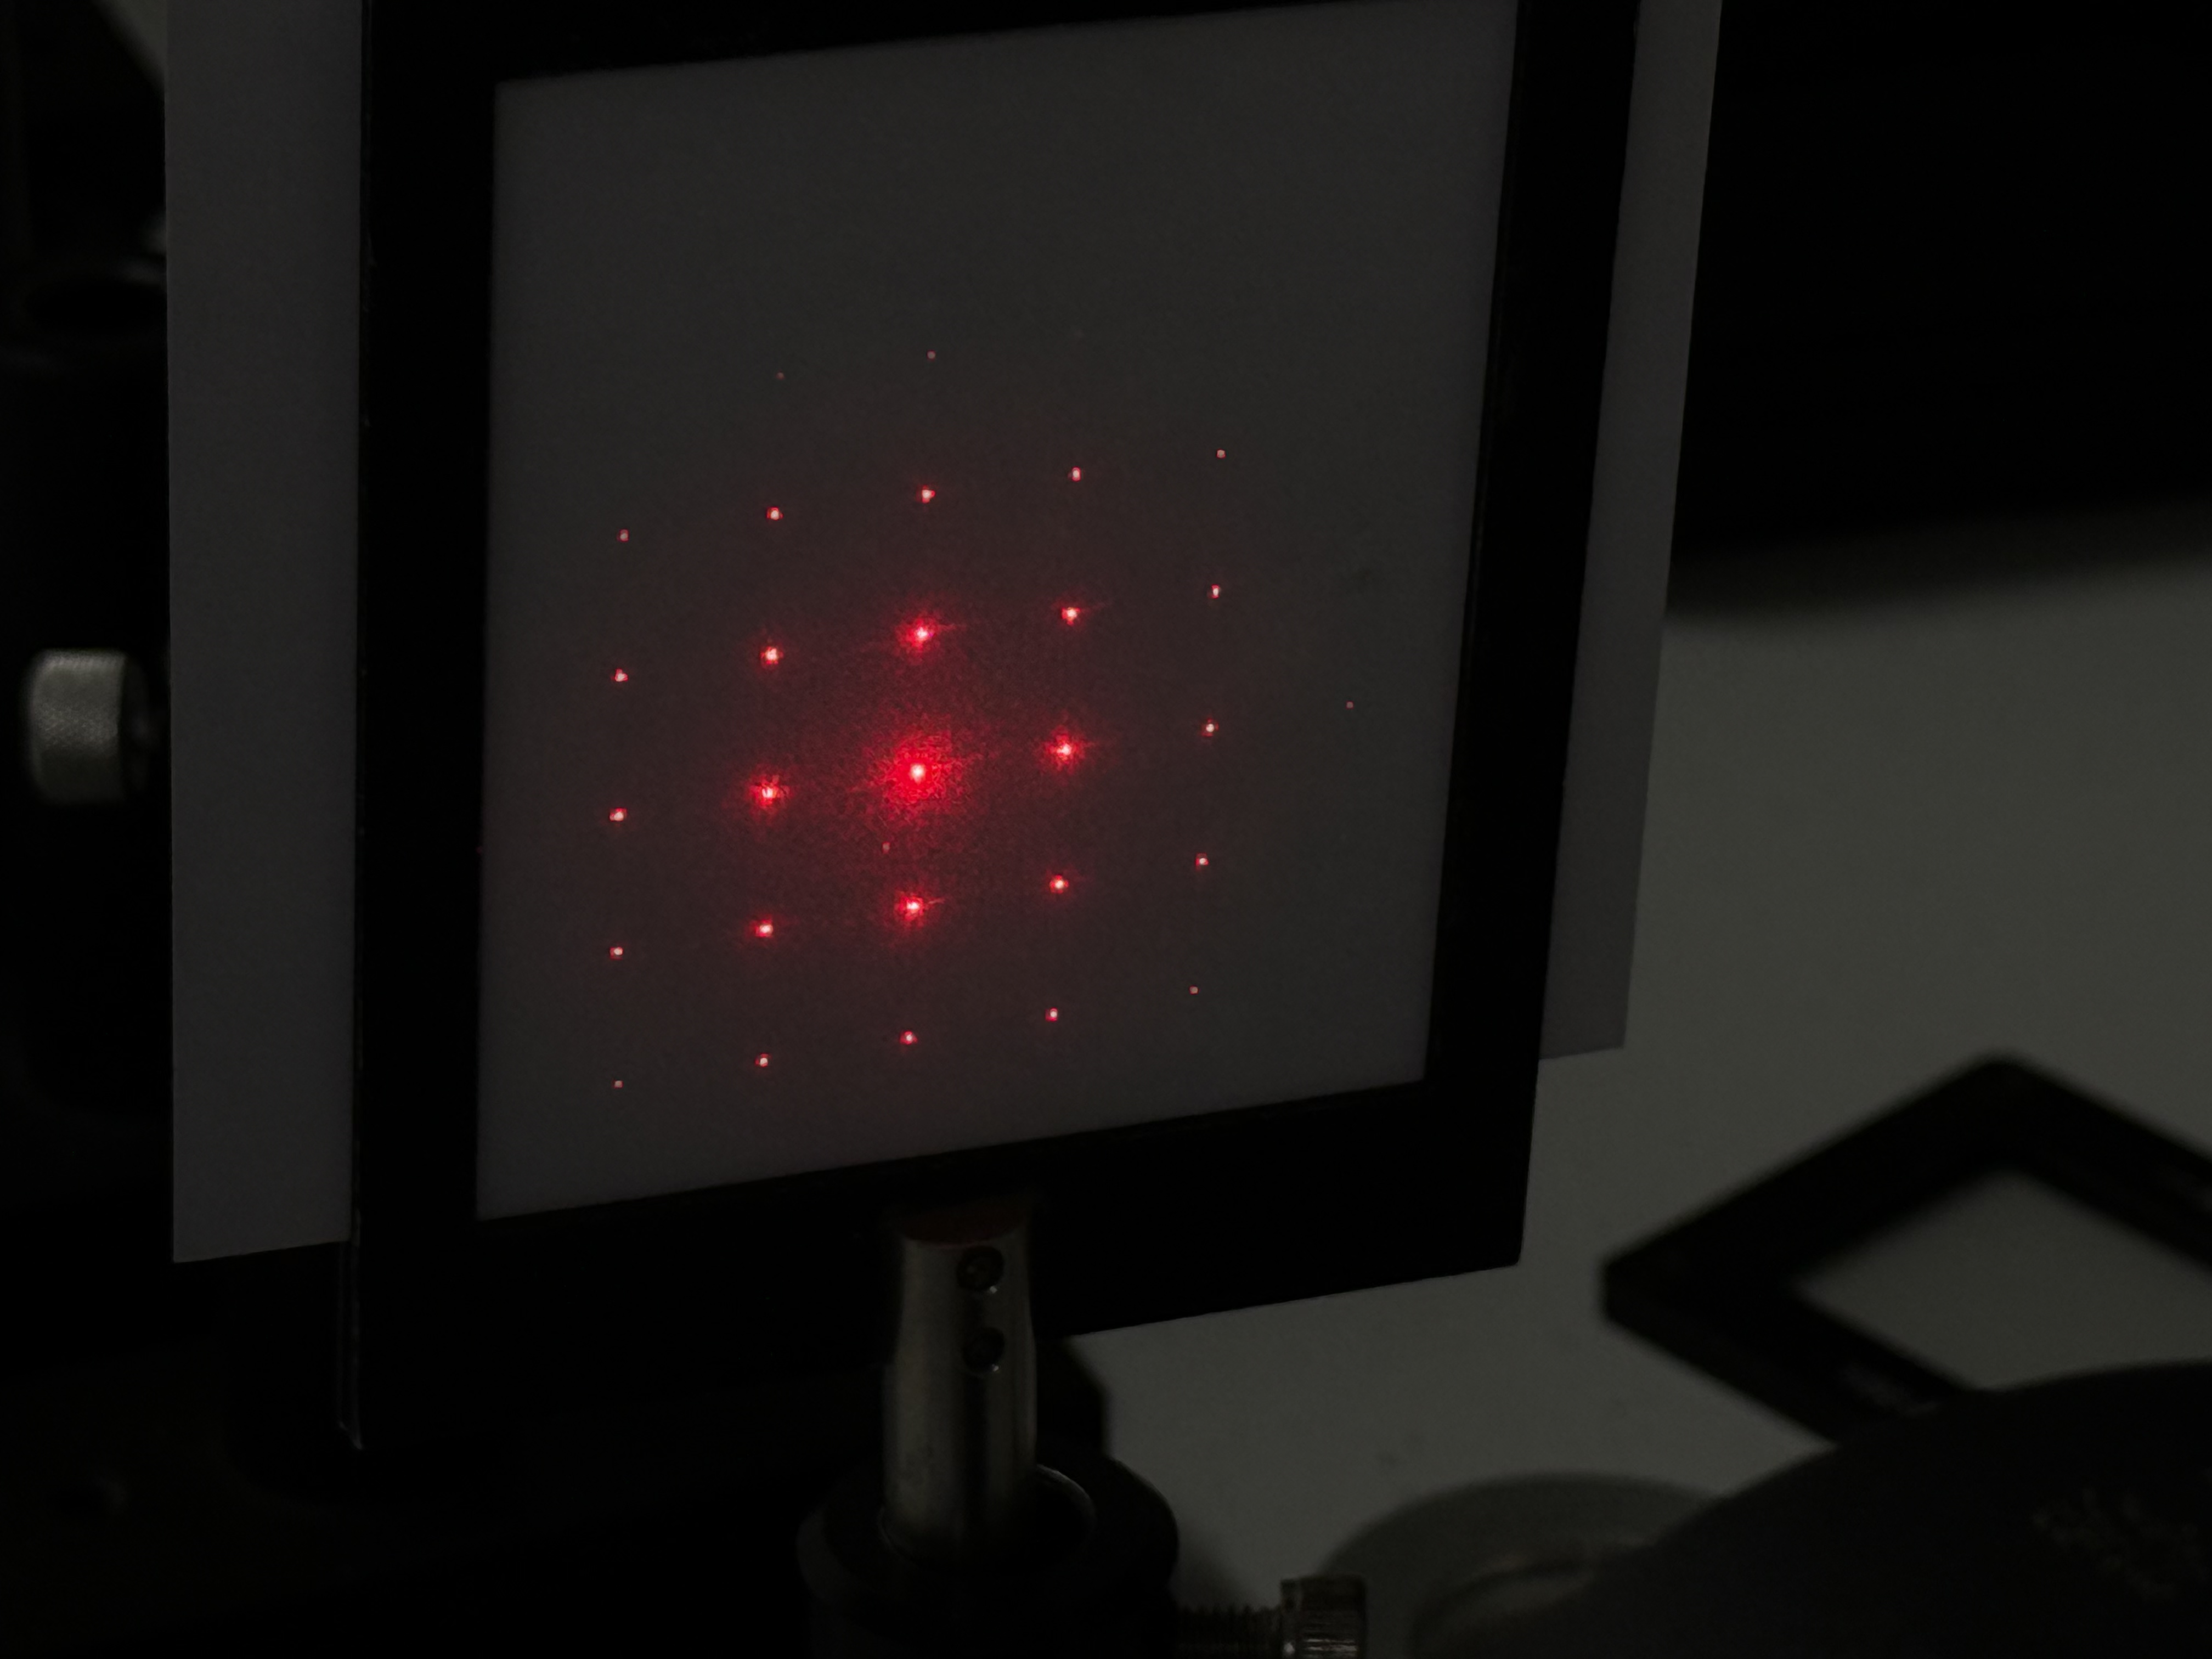
\includegraphics[width=0.9\textwidth]{Data/003-pattern/conv_base_1.png}
        \subcaption{卷积件1}
        \label{fig:convolution_base_1}
    \end{subfigure}

    \begin{subfigure}[b]{0.4\textwidth}
        \centering
        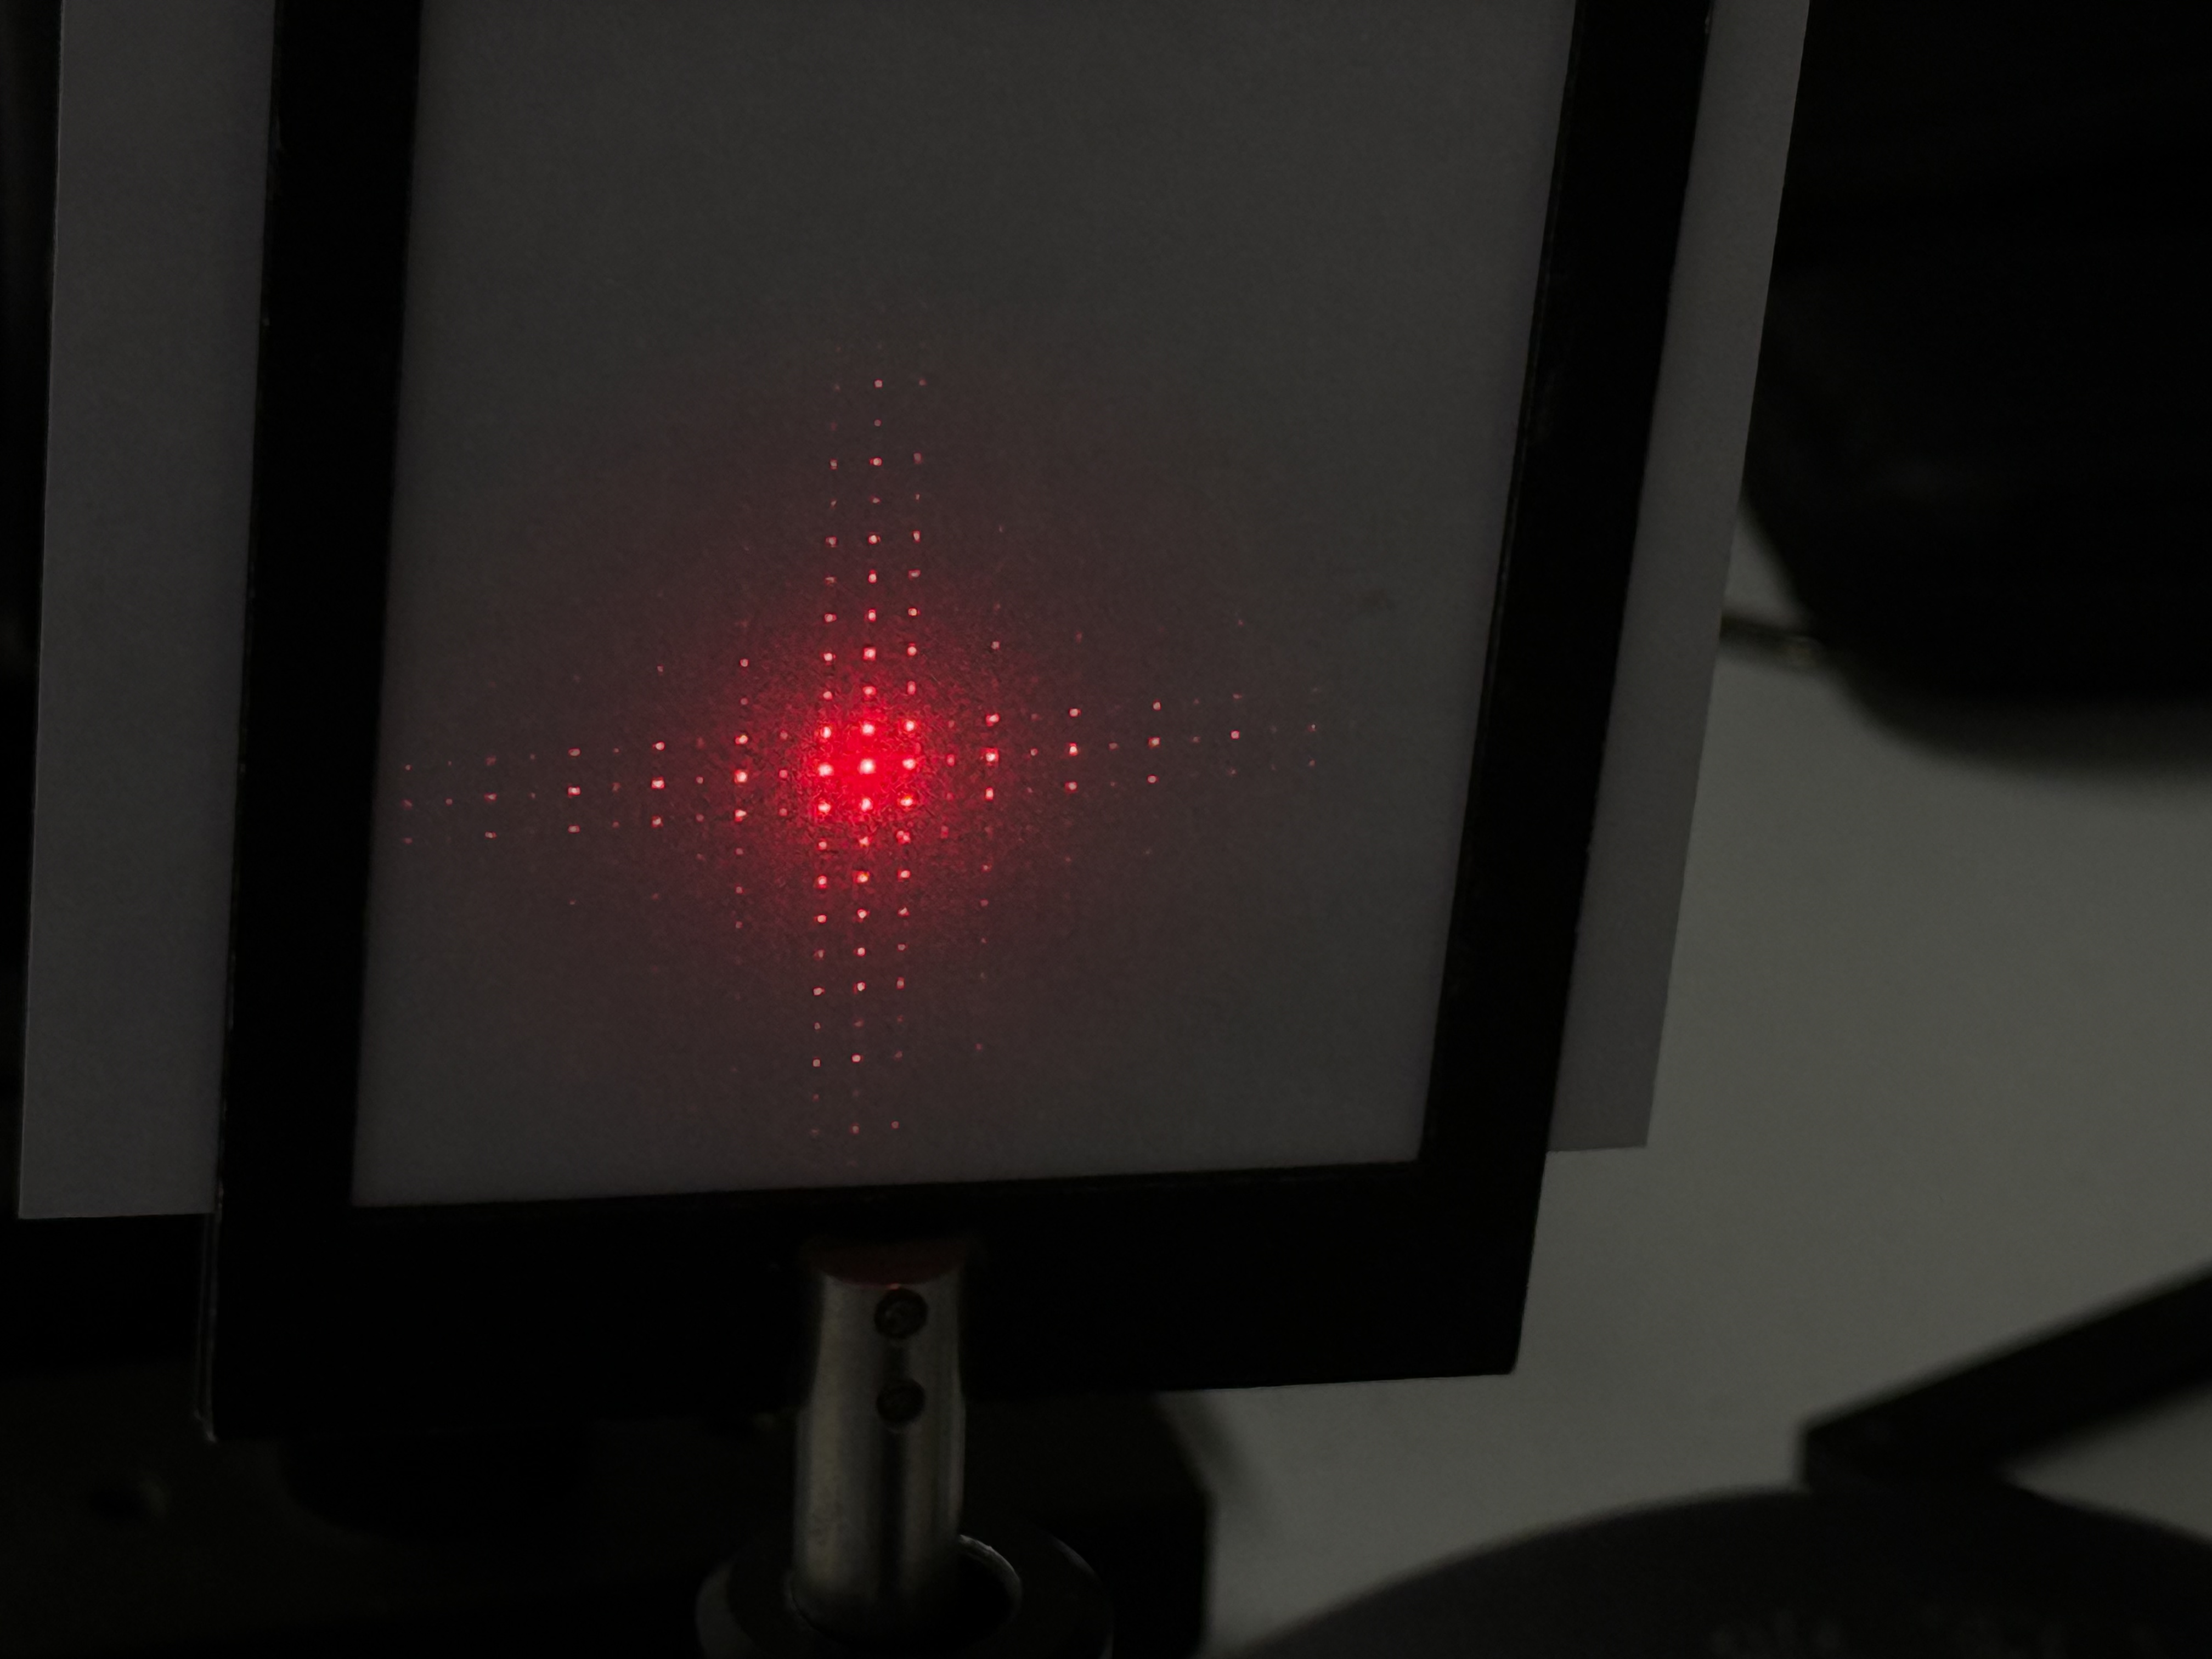
\includegraphics[width=0.9\textwidth]{Data/003-pattern/conv_base_2.png}
        \subcaption{卷积件2}
        \label{fig:convolution_base_2}
    \end{subfigure}

    \caption{卷积件单独放置所得衍射图样}
    \captionnamefont{\wuhao\bf\heiti}
    \captiontitlefont{\wuhao\bf\heiti}
    \label{fig:convolution_base}
\end{figure*}

\begin{figure*}
    \centering
    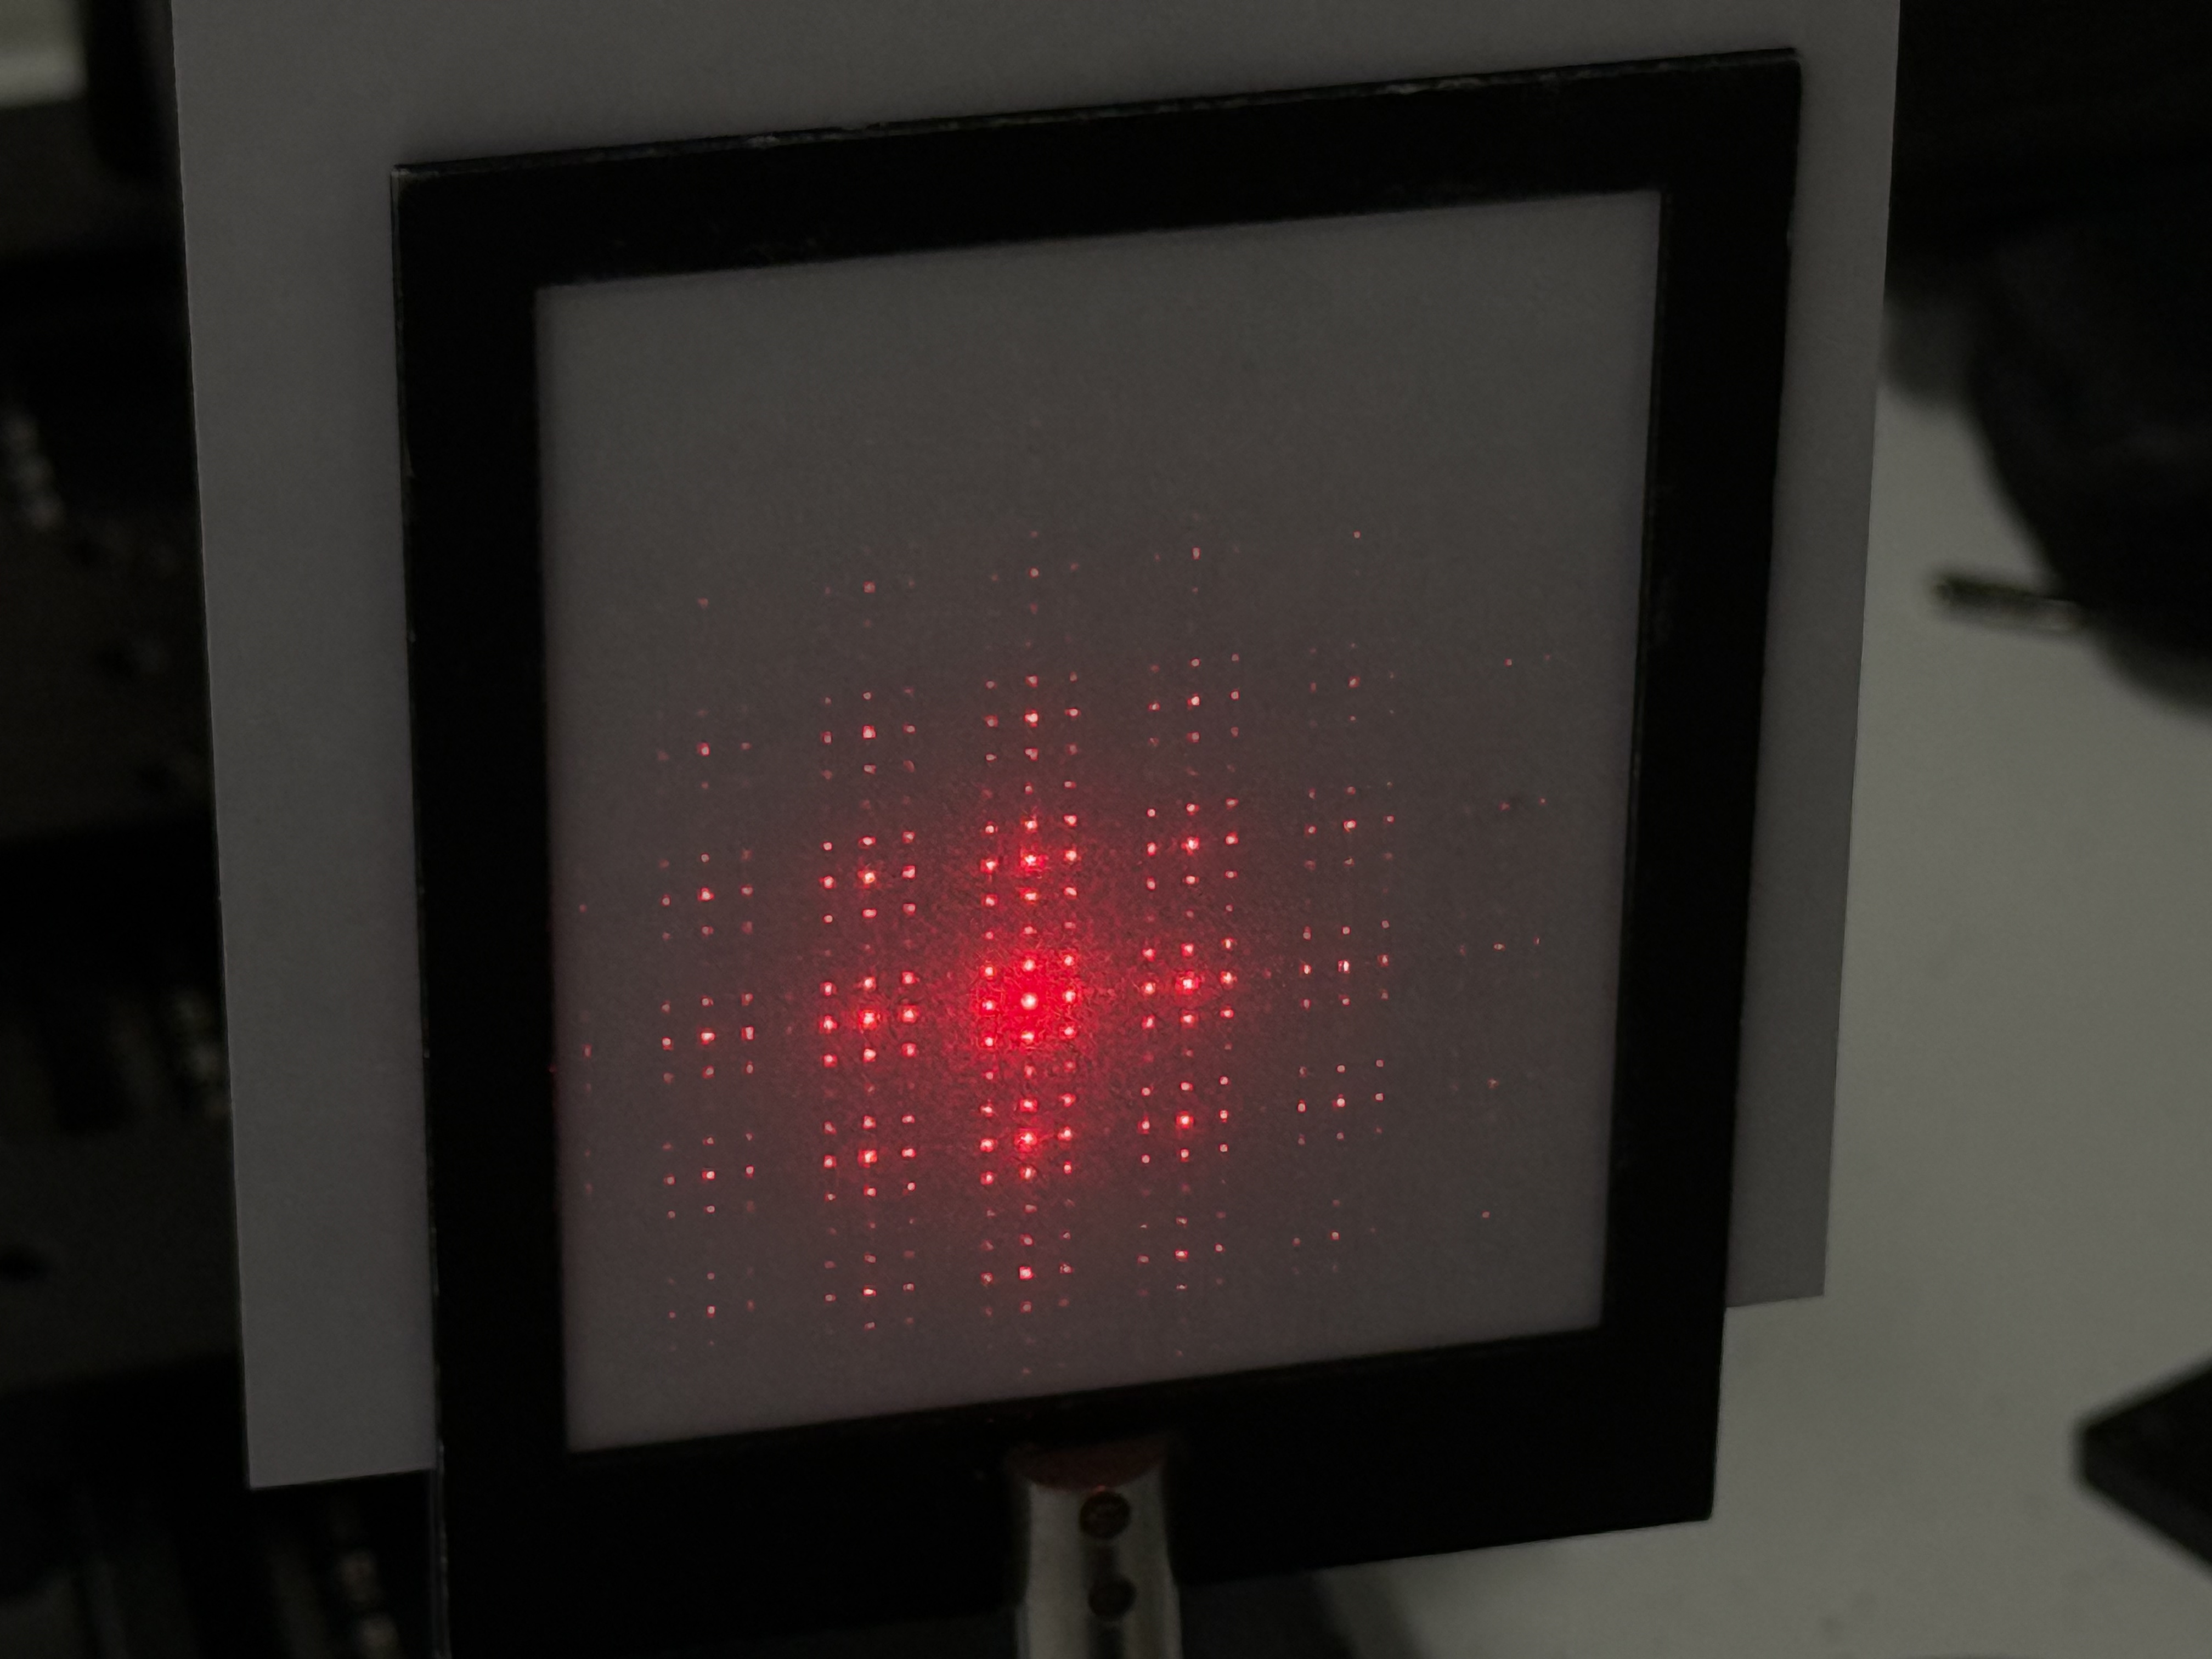
\includegraphics[width=0.9\textwidth]{Data/003-pattern/conv_344_164.png}
    \caption{卷积件密接同向放置所得衍射图样}
    \label{fig:convolution_result}
\end{figure*}

将两块卷积件各自置于频谱面,在像面可观测到二维点阵的衍射图样,如图\ref{fig:convolution_base}所示;在两块卷积件密接同向放置时,如图\ref{fig:convolution_result}所示,能够观察到卷积件2对应的较为细密的衍射图样,以卷积件1衍射图样对应的空间周期以及方向进行排布,并可估计卷积件1, 2光栅常数$d_{1,2}$有以下关系:

\begin{equation}
    d_1 : d_2 \approx 1 : 4
\end{equation}

% 卷积件1依次转过0, 30, 45, 60, 90度,五张图“上三下二”排布
\begin{figure*}
    \centering
    \begin{subfigure}[b]{0.3\textwidth}
        \centering
        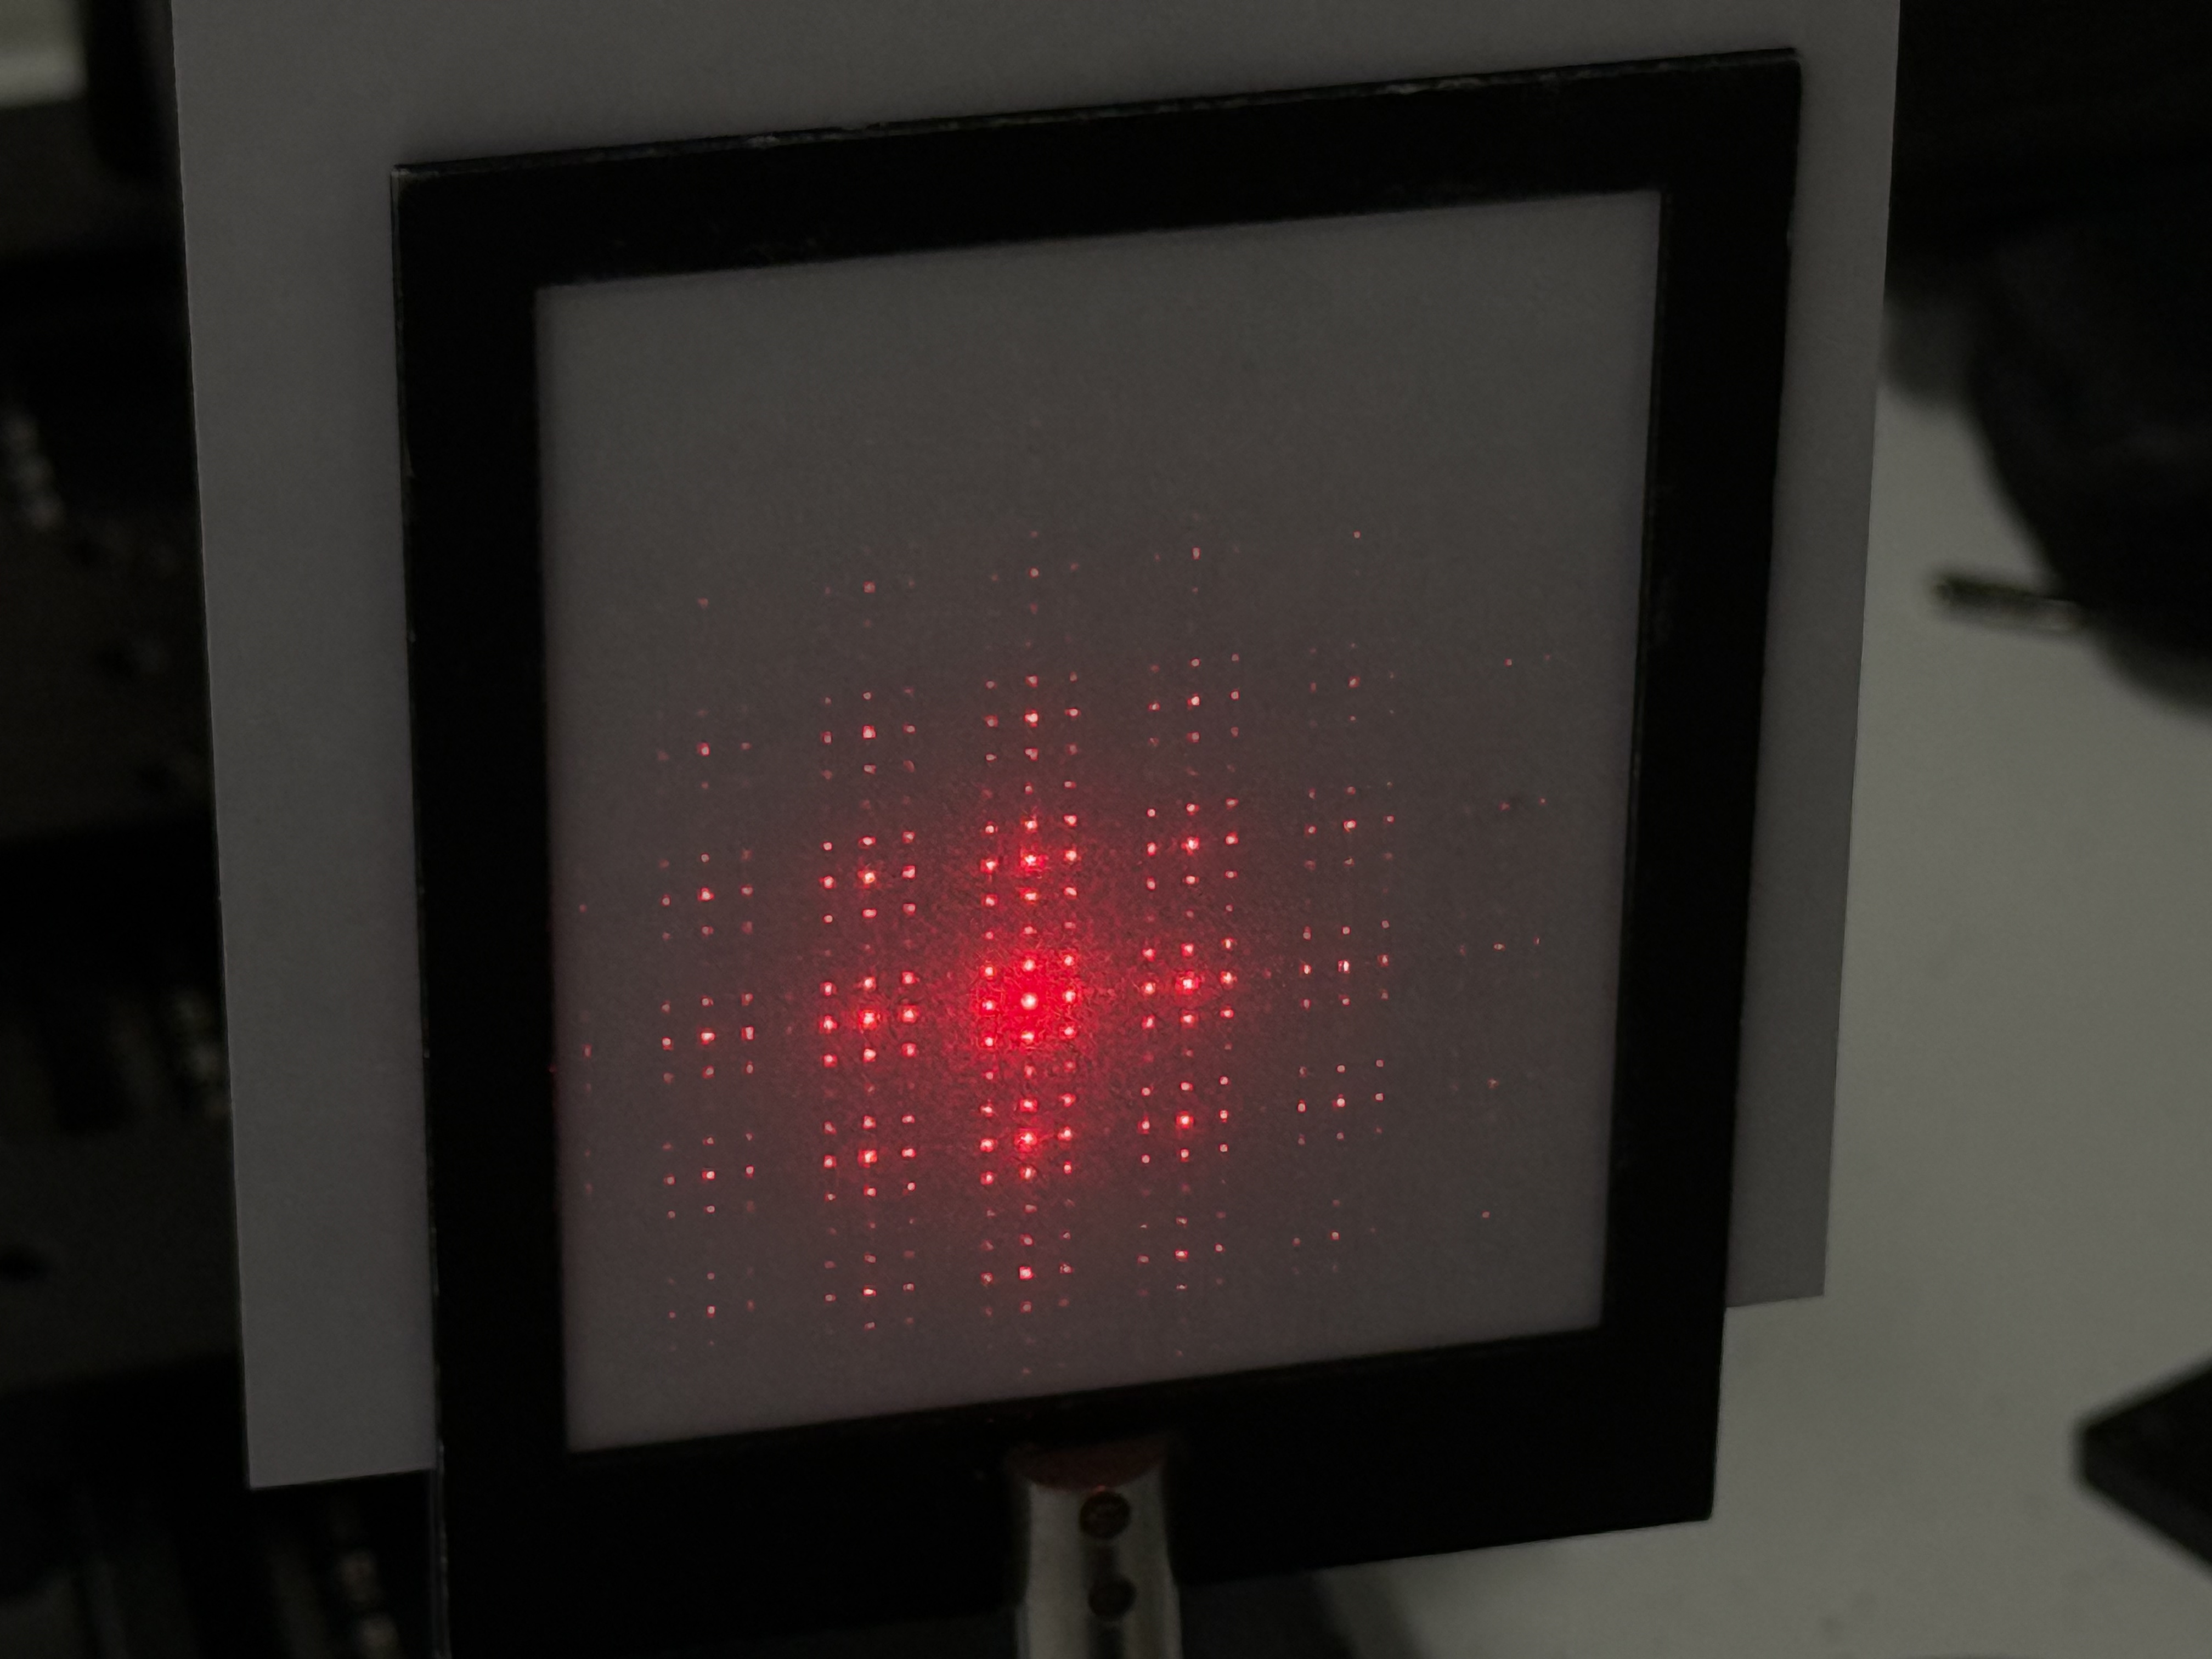
\includegraphics[width=0.9\textwidth]{Data/003-pattern/conv_344_164.png}
        \subcaption{$+0^\circ$}
        \label{fig:convolution_rot_01_00deg}
    \end{subfigure}% 
    \hspace{0.03\textwidth}% --- 固定的水平间距 ---
    \begin{subfigure}[b]{0.3\textwidth}
        \centering
        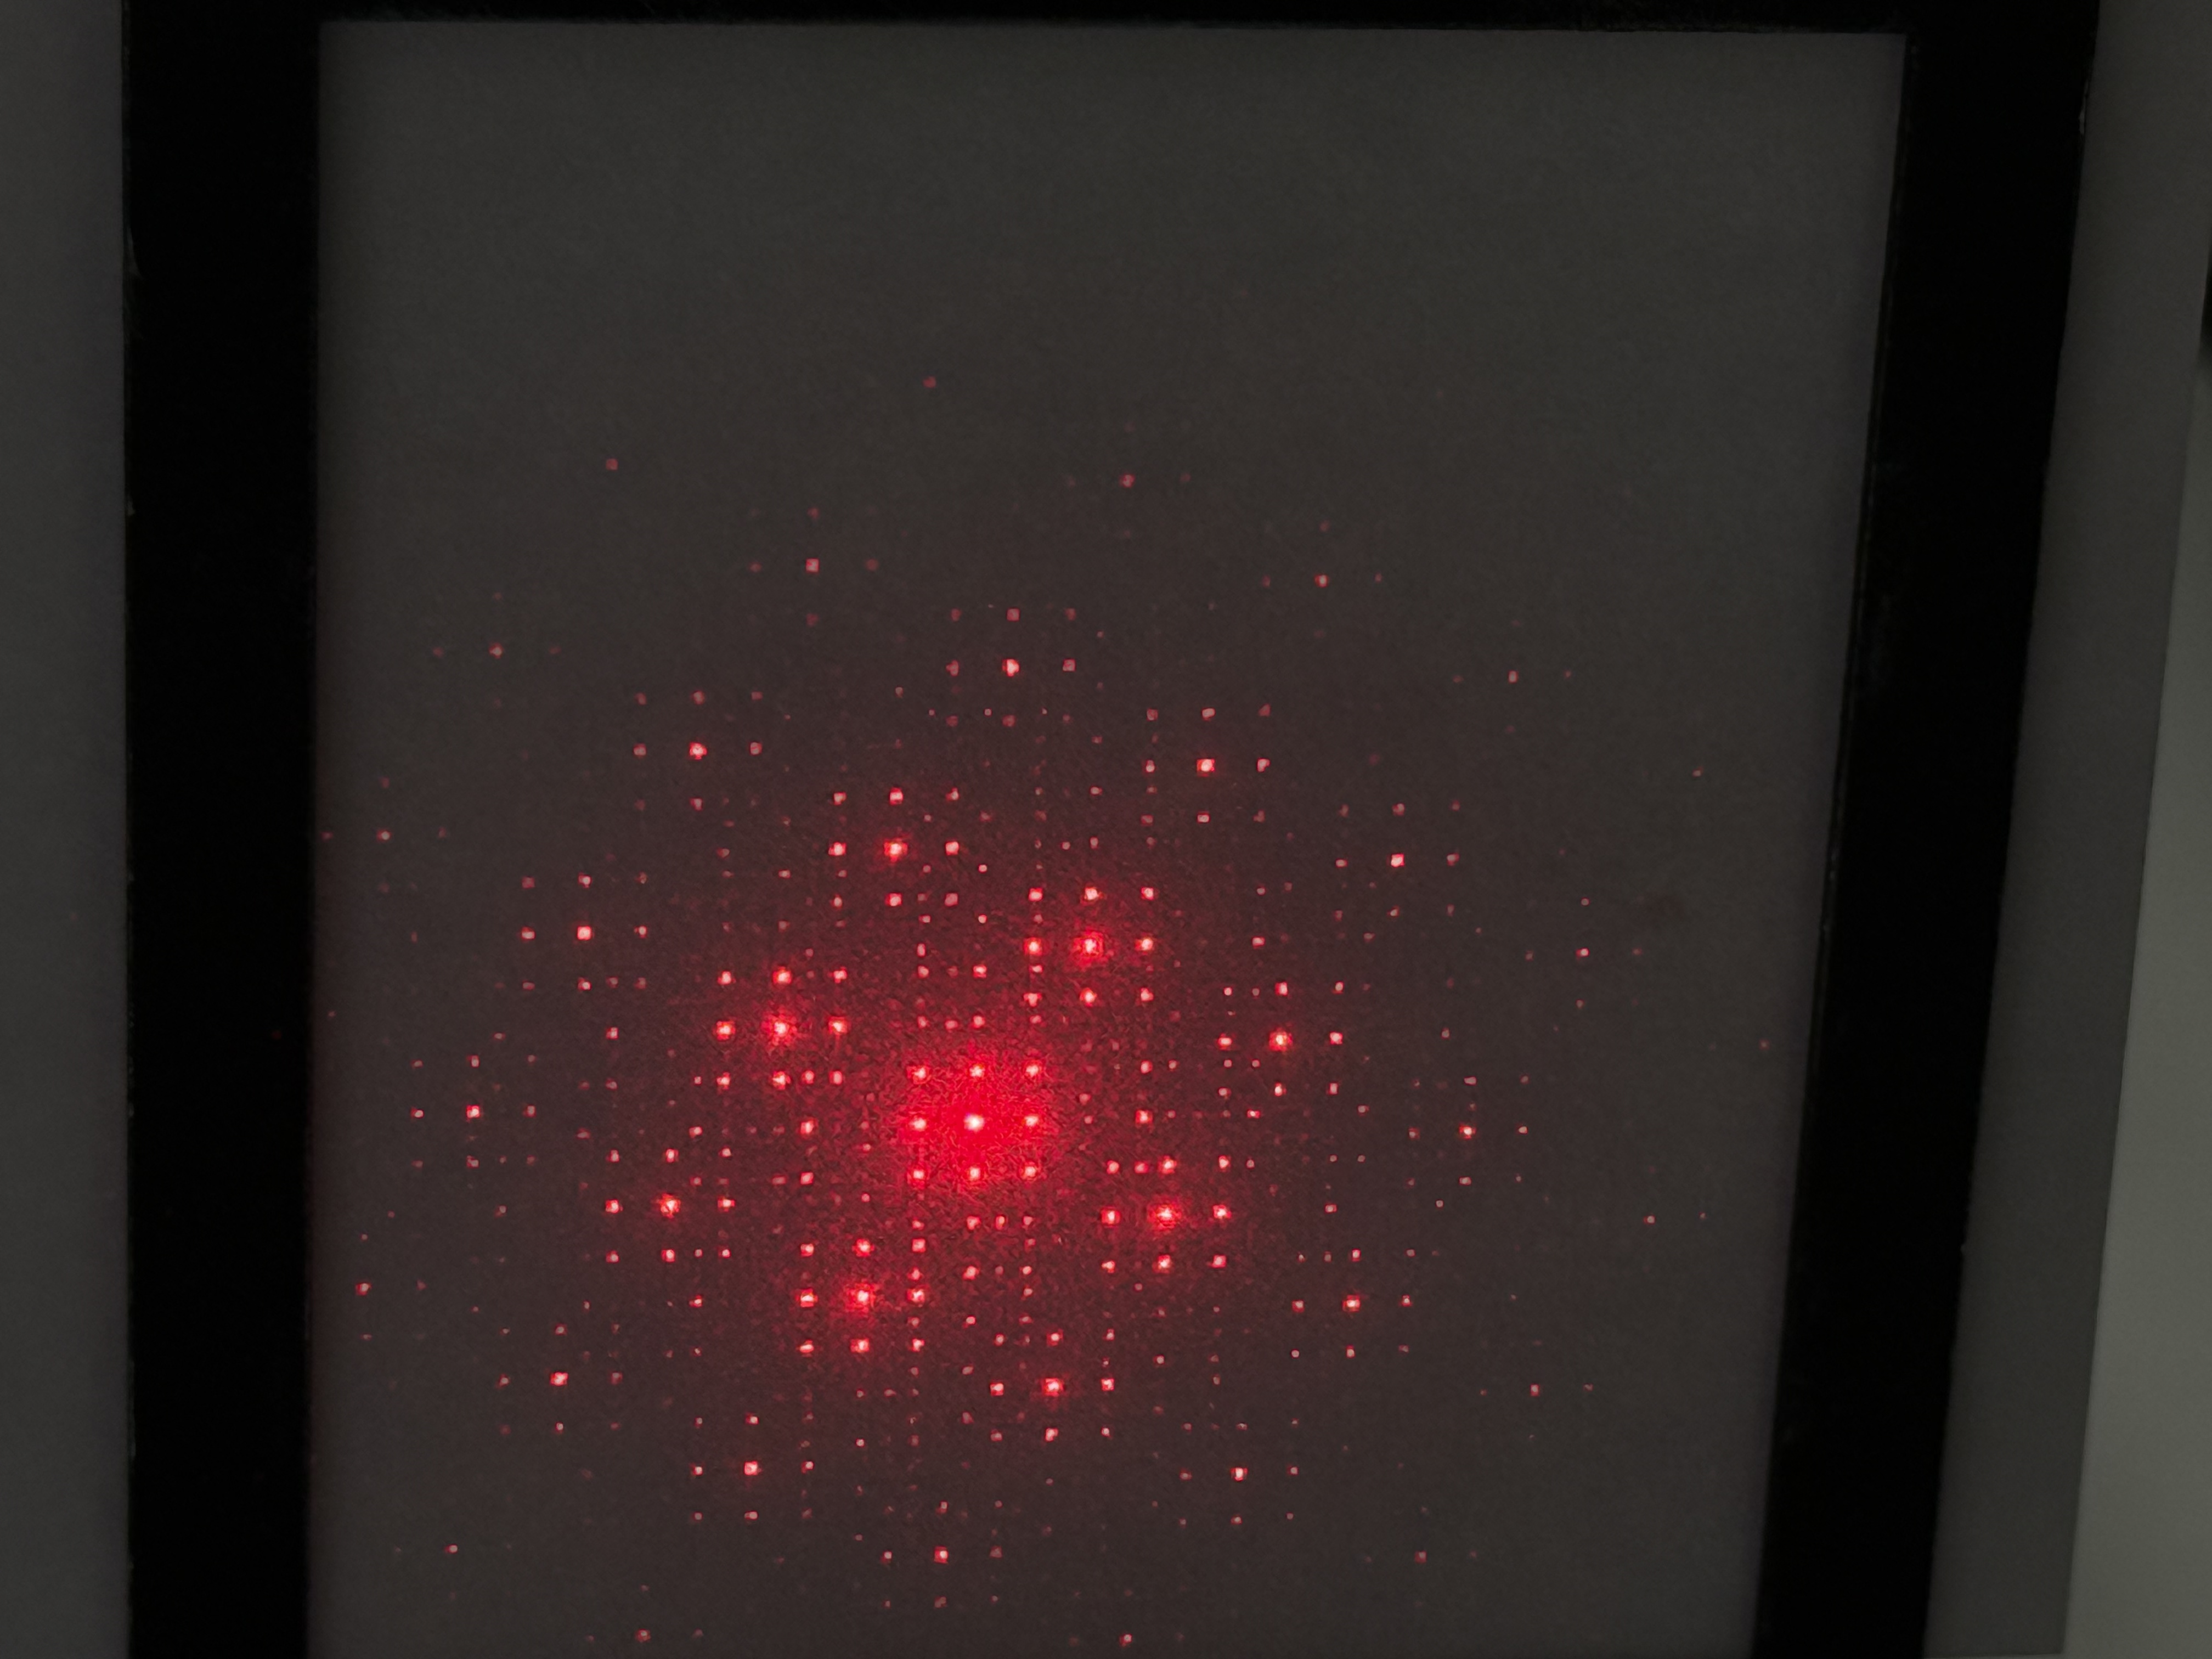
\includegraphics[width=0.9\textwidth]{Data/003-pattern/conv_014_164.png}
        \subcaption{$+30^\circ$}
        \label{fig:convolution_rot_01_30deg}
    \end{subfigure}%
    \hspace{0.03\textwidth}% --- 固定的水平间距 ---
    \begin{subfigure}[b]{0.3\textwidth}
        \centering
        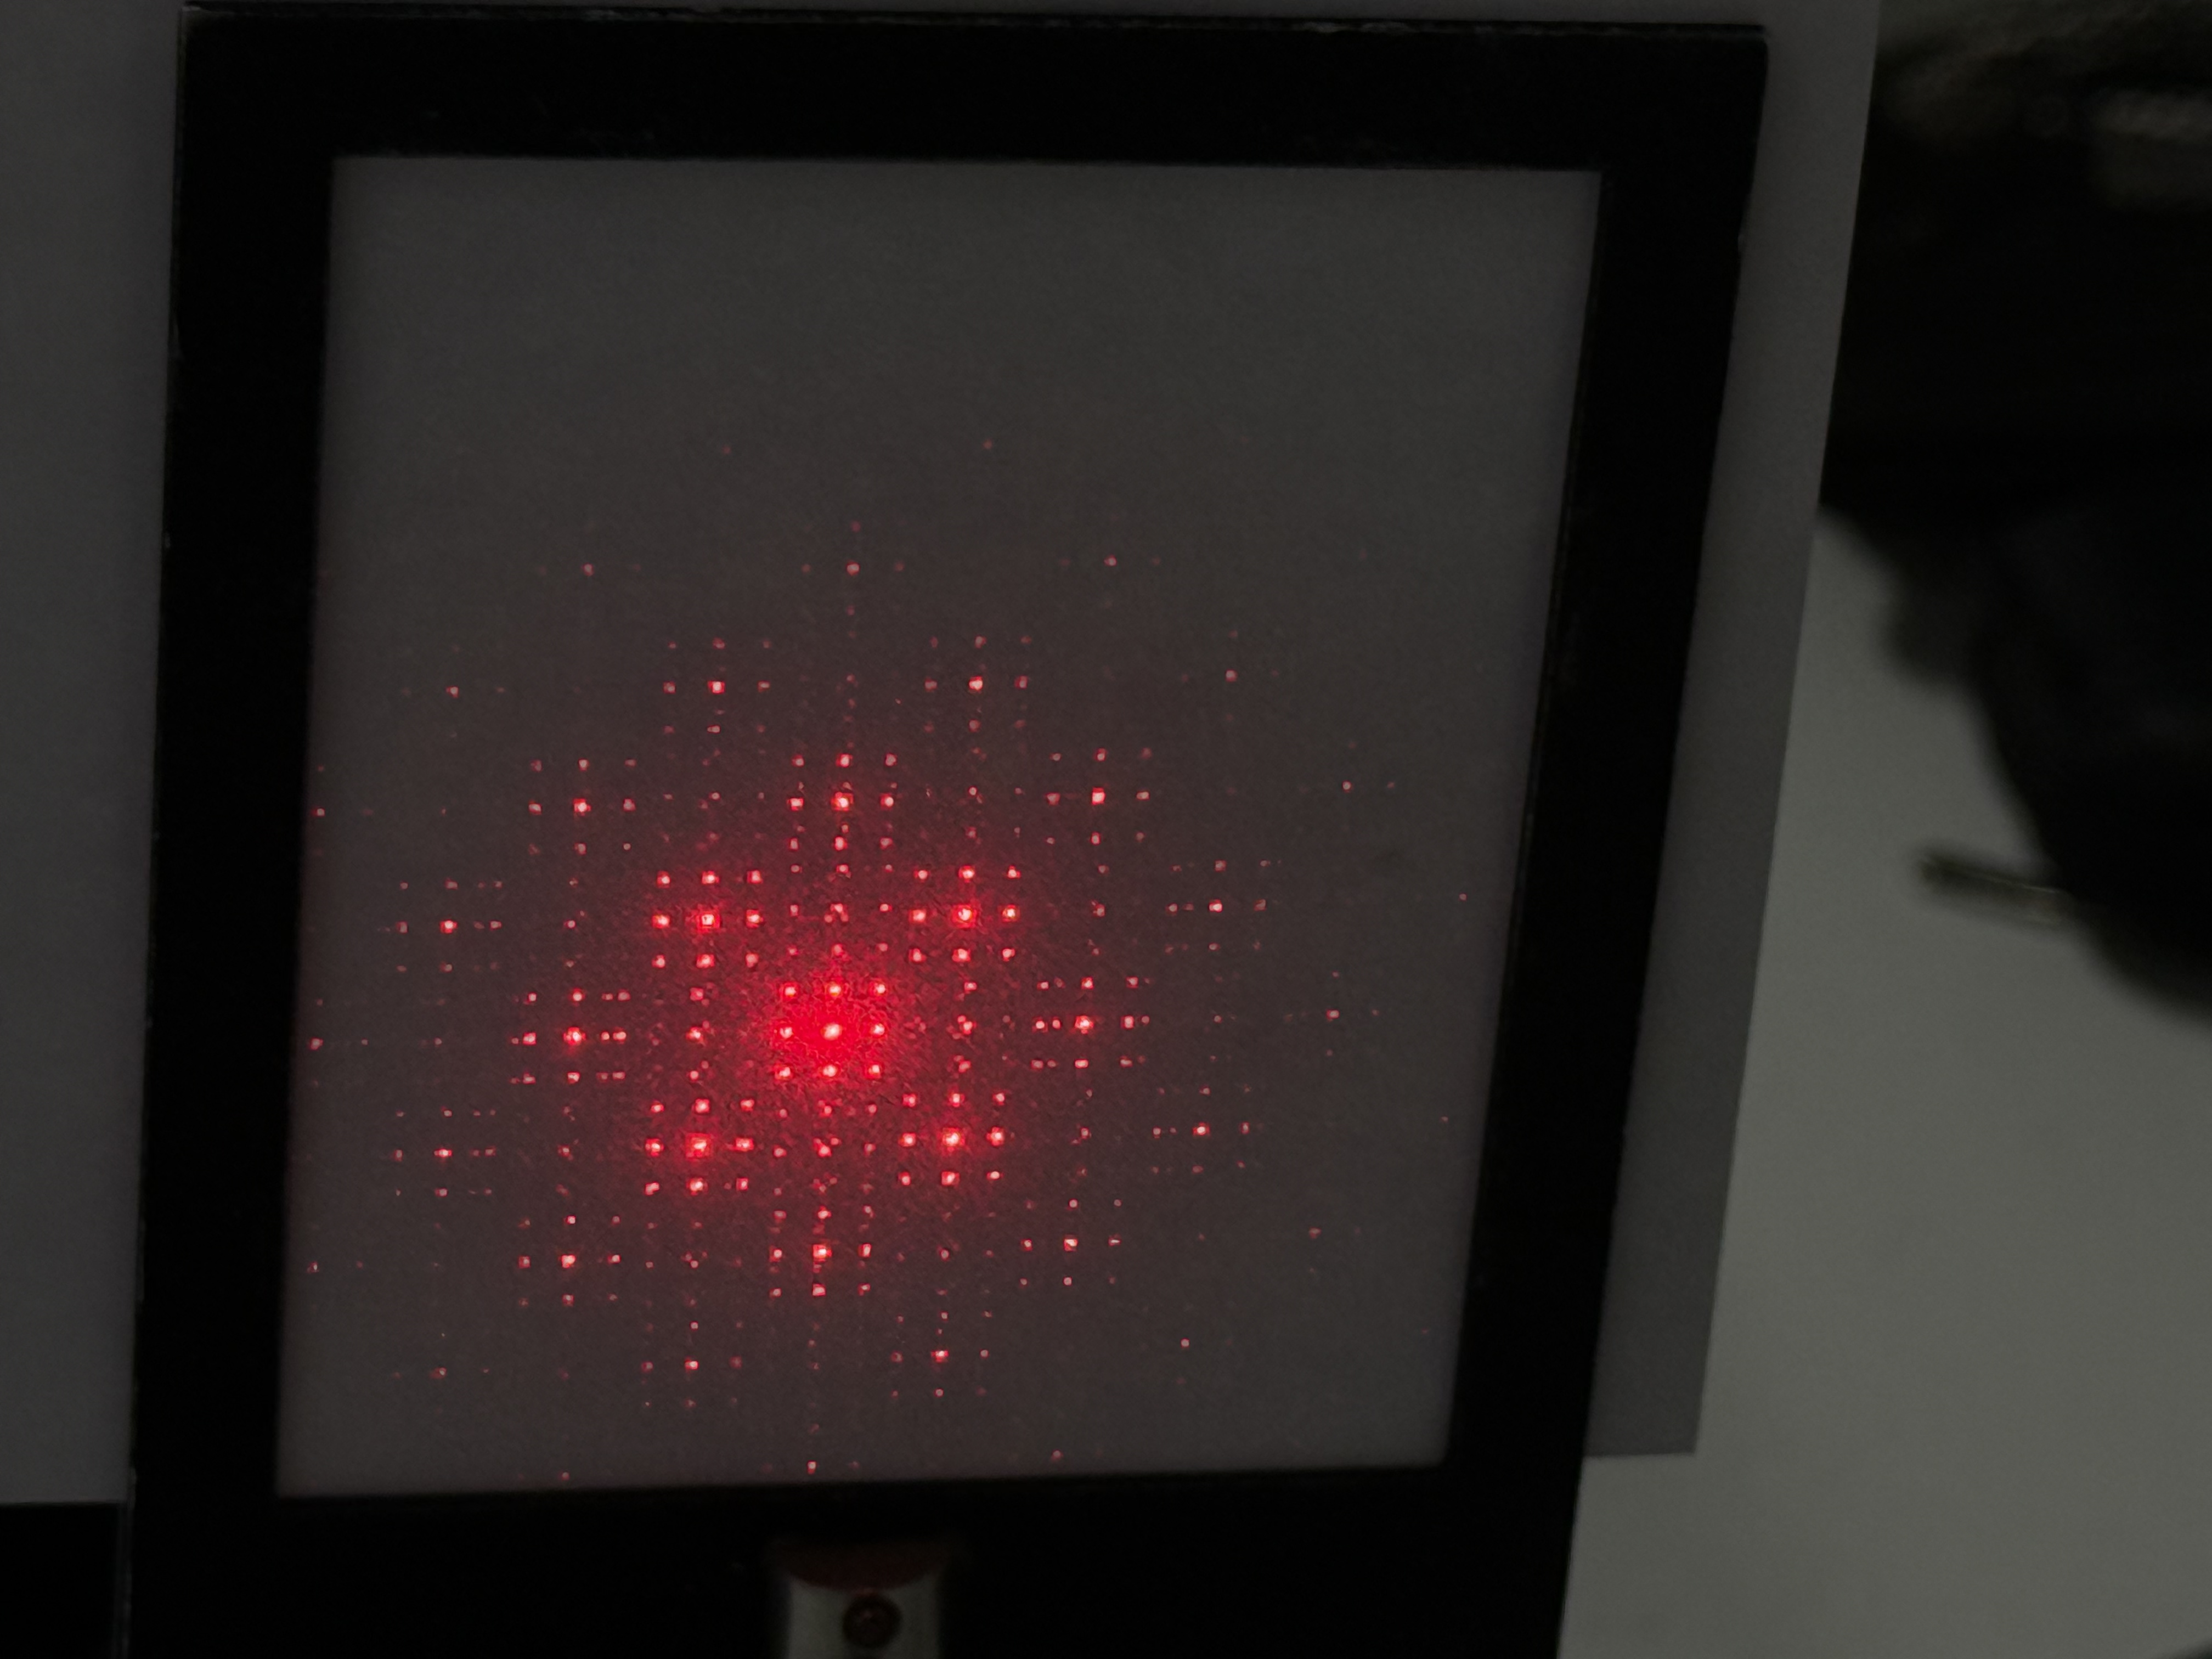
\includegraphics[width=0.9\textwidth]{Data/003-pattern/conv_029_164.png}
        \subcaption{$+45^\circ$}
        \label{fig:convolution_rot_01_45deg}
    \end{subfigure}
    
    % --- 换行并添加垂直间距 ---
    \vspace{1em}
    
    % --- 第二排:2张图 ---
    % 由于外层有 \centering,这两张图会自动整体居中
    \begin{subfigure}[b]{0.3\textwidth}
        \centering
        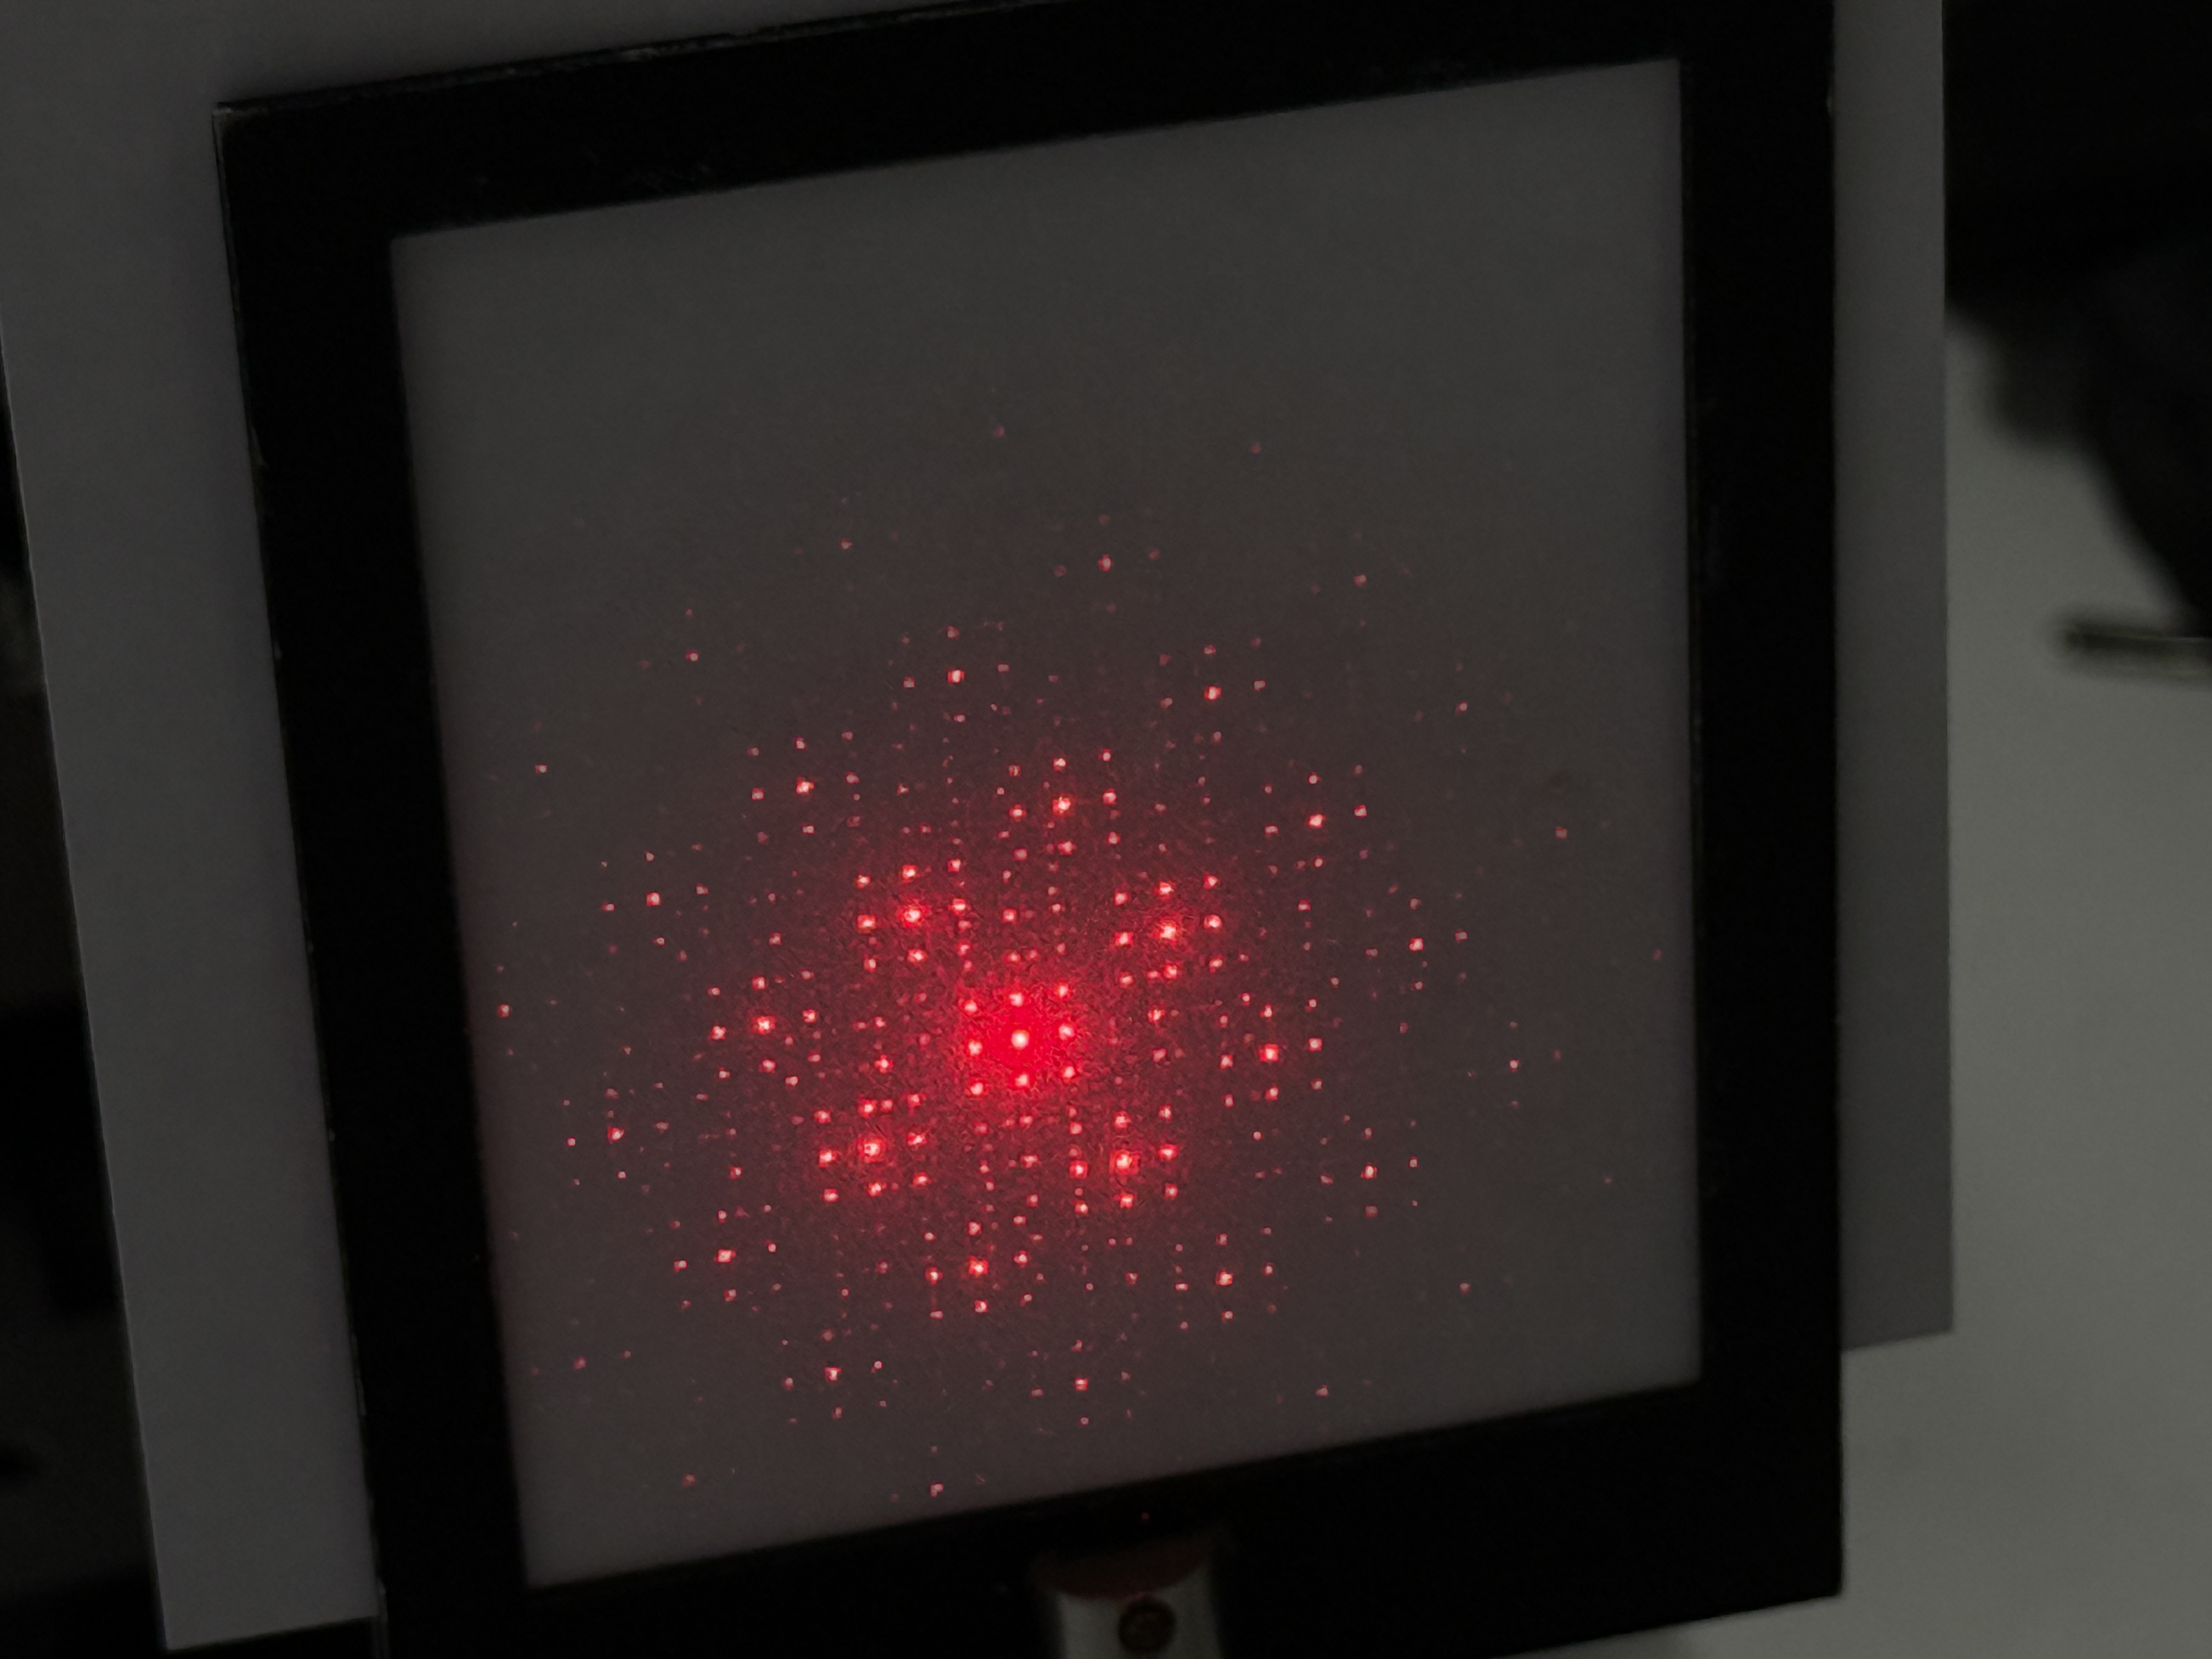
\includegraphics[width=0.9\textwidth]{Data/003-pattern/conv_044_164.png}
        \subcaption{$+60^\circ$}
        \label{fig:convolution_rot_01_60deg}
    \end{subfigure}%
    \hspace{0.03\textwidth}% --- 必须与第一排间距完全一致 ---
    \begin{subfigure}[b]{0.3\textwidth}
        \centering
        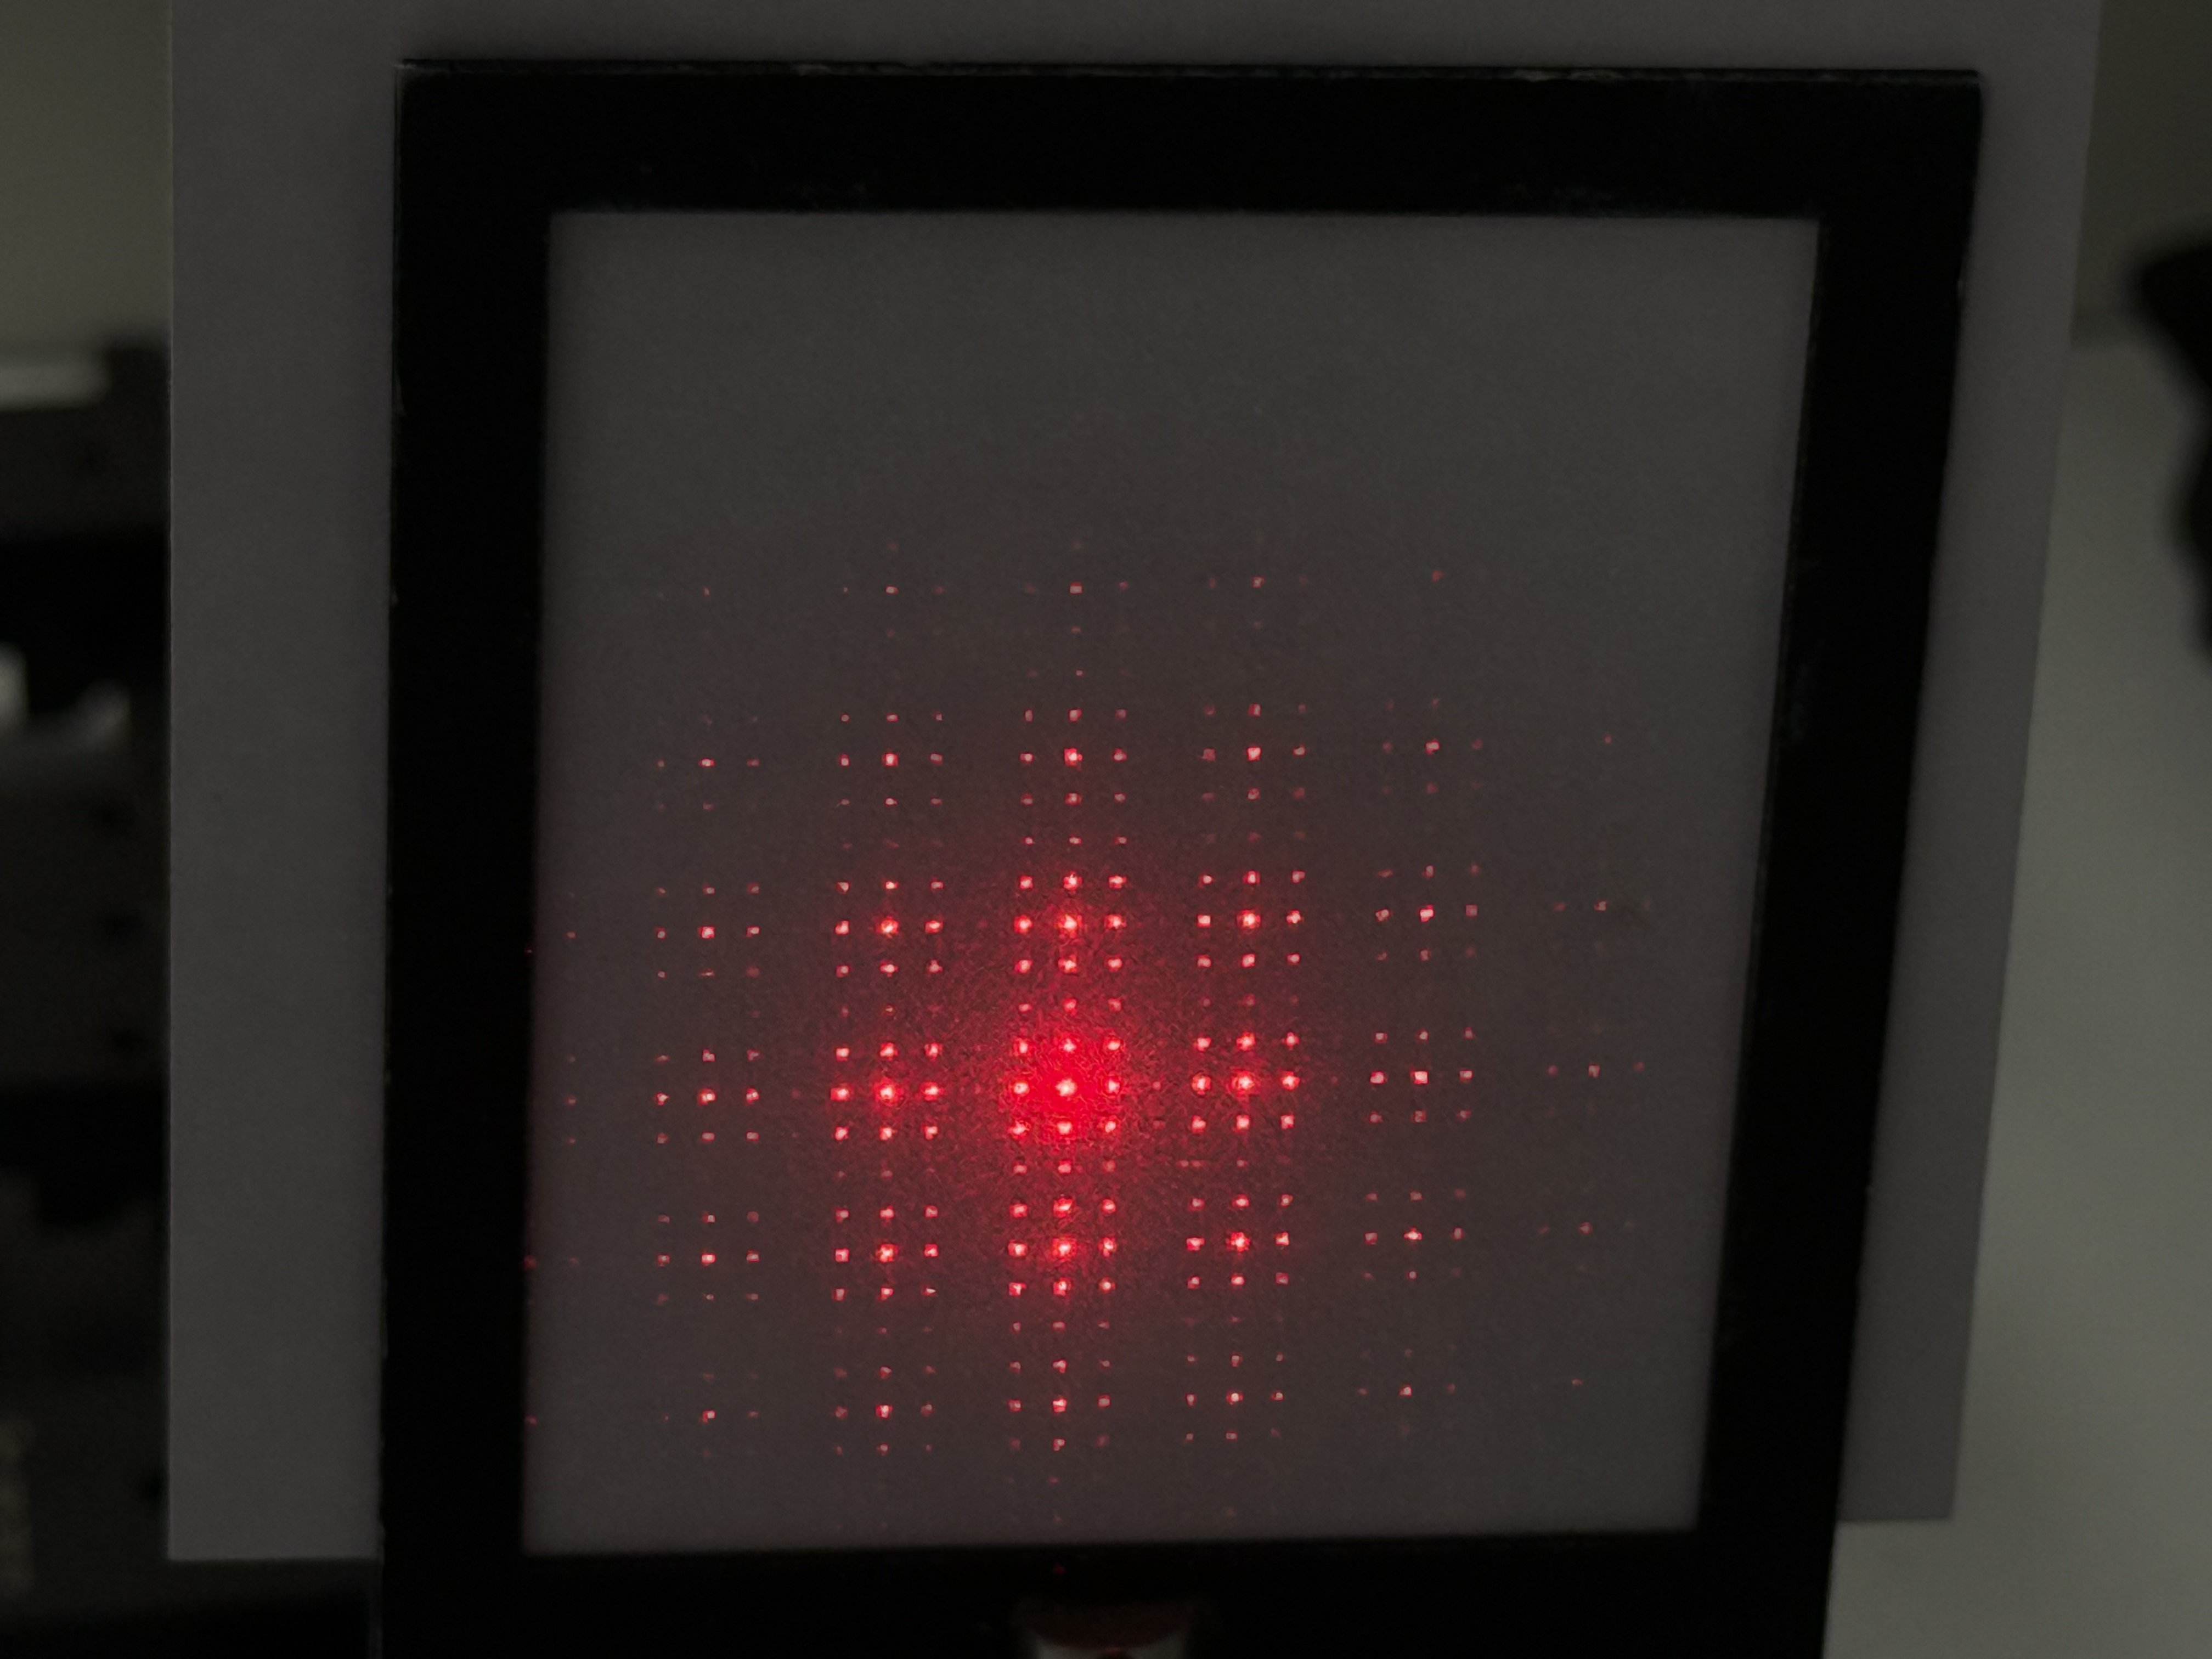
\includegraphics[width=0.9\textwidth]{Data/003-pattern/conv_074_164.png}
        \subcaption{$+90^\circ$}
        \label{fig:convolution_rot_01_90deg}
    \end{subfigure}
    \caption{单独旋转卷积件1至不同角度所得衍射图样}
    \captionnamefont{\wuhao\bf\heiti}
    \captiontitlefont{\wuhao\bf\heiti}
    \label{fig:convolution_rot_01}
\end{figure*}

先后单独转动卷积件1至一系列不同角度,可观察到:与卷积件2相关联的小周期衍射图样整体形貌、取向以及周期均未发生显著变化;这些小周期衍射图样排布的取向则伴随卷积件1的旋转而变化。

% 卷积件2依次转过0, 30, 45, 60, 90度,五张图“上三下二”排布
\begin{figure*}
    \centering
    \begin{subfigure}[b]{0.3\textwidth}
        \centering
        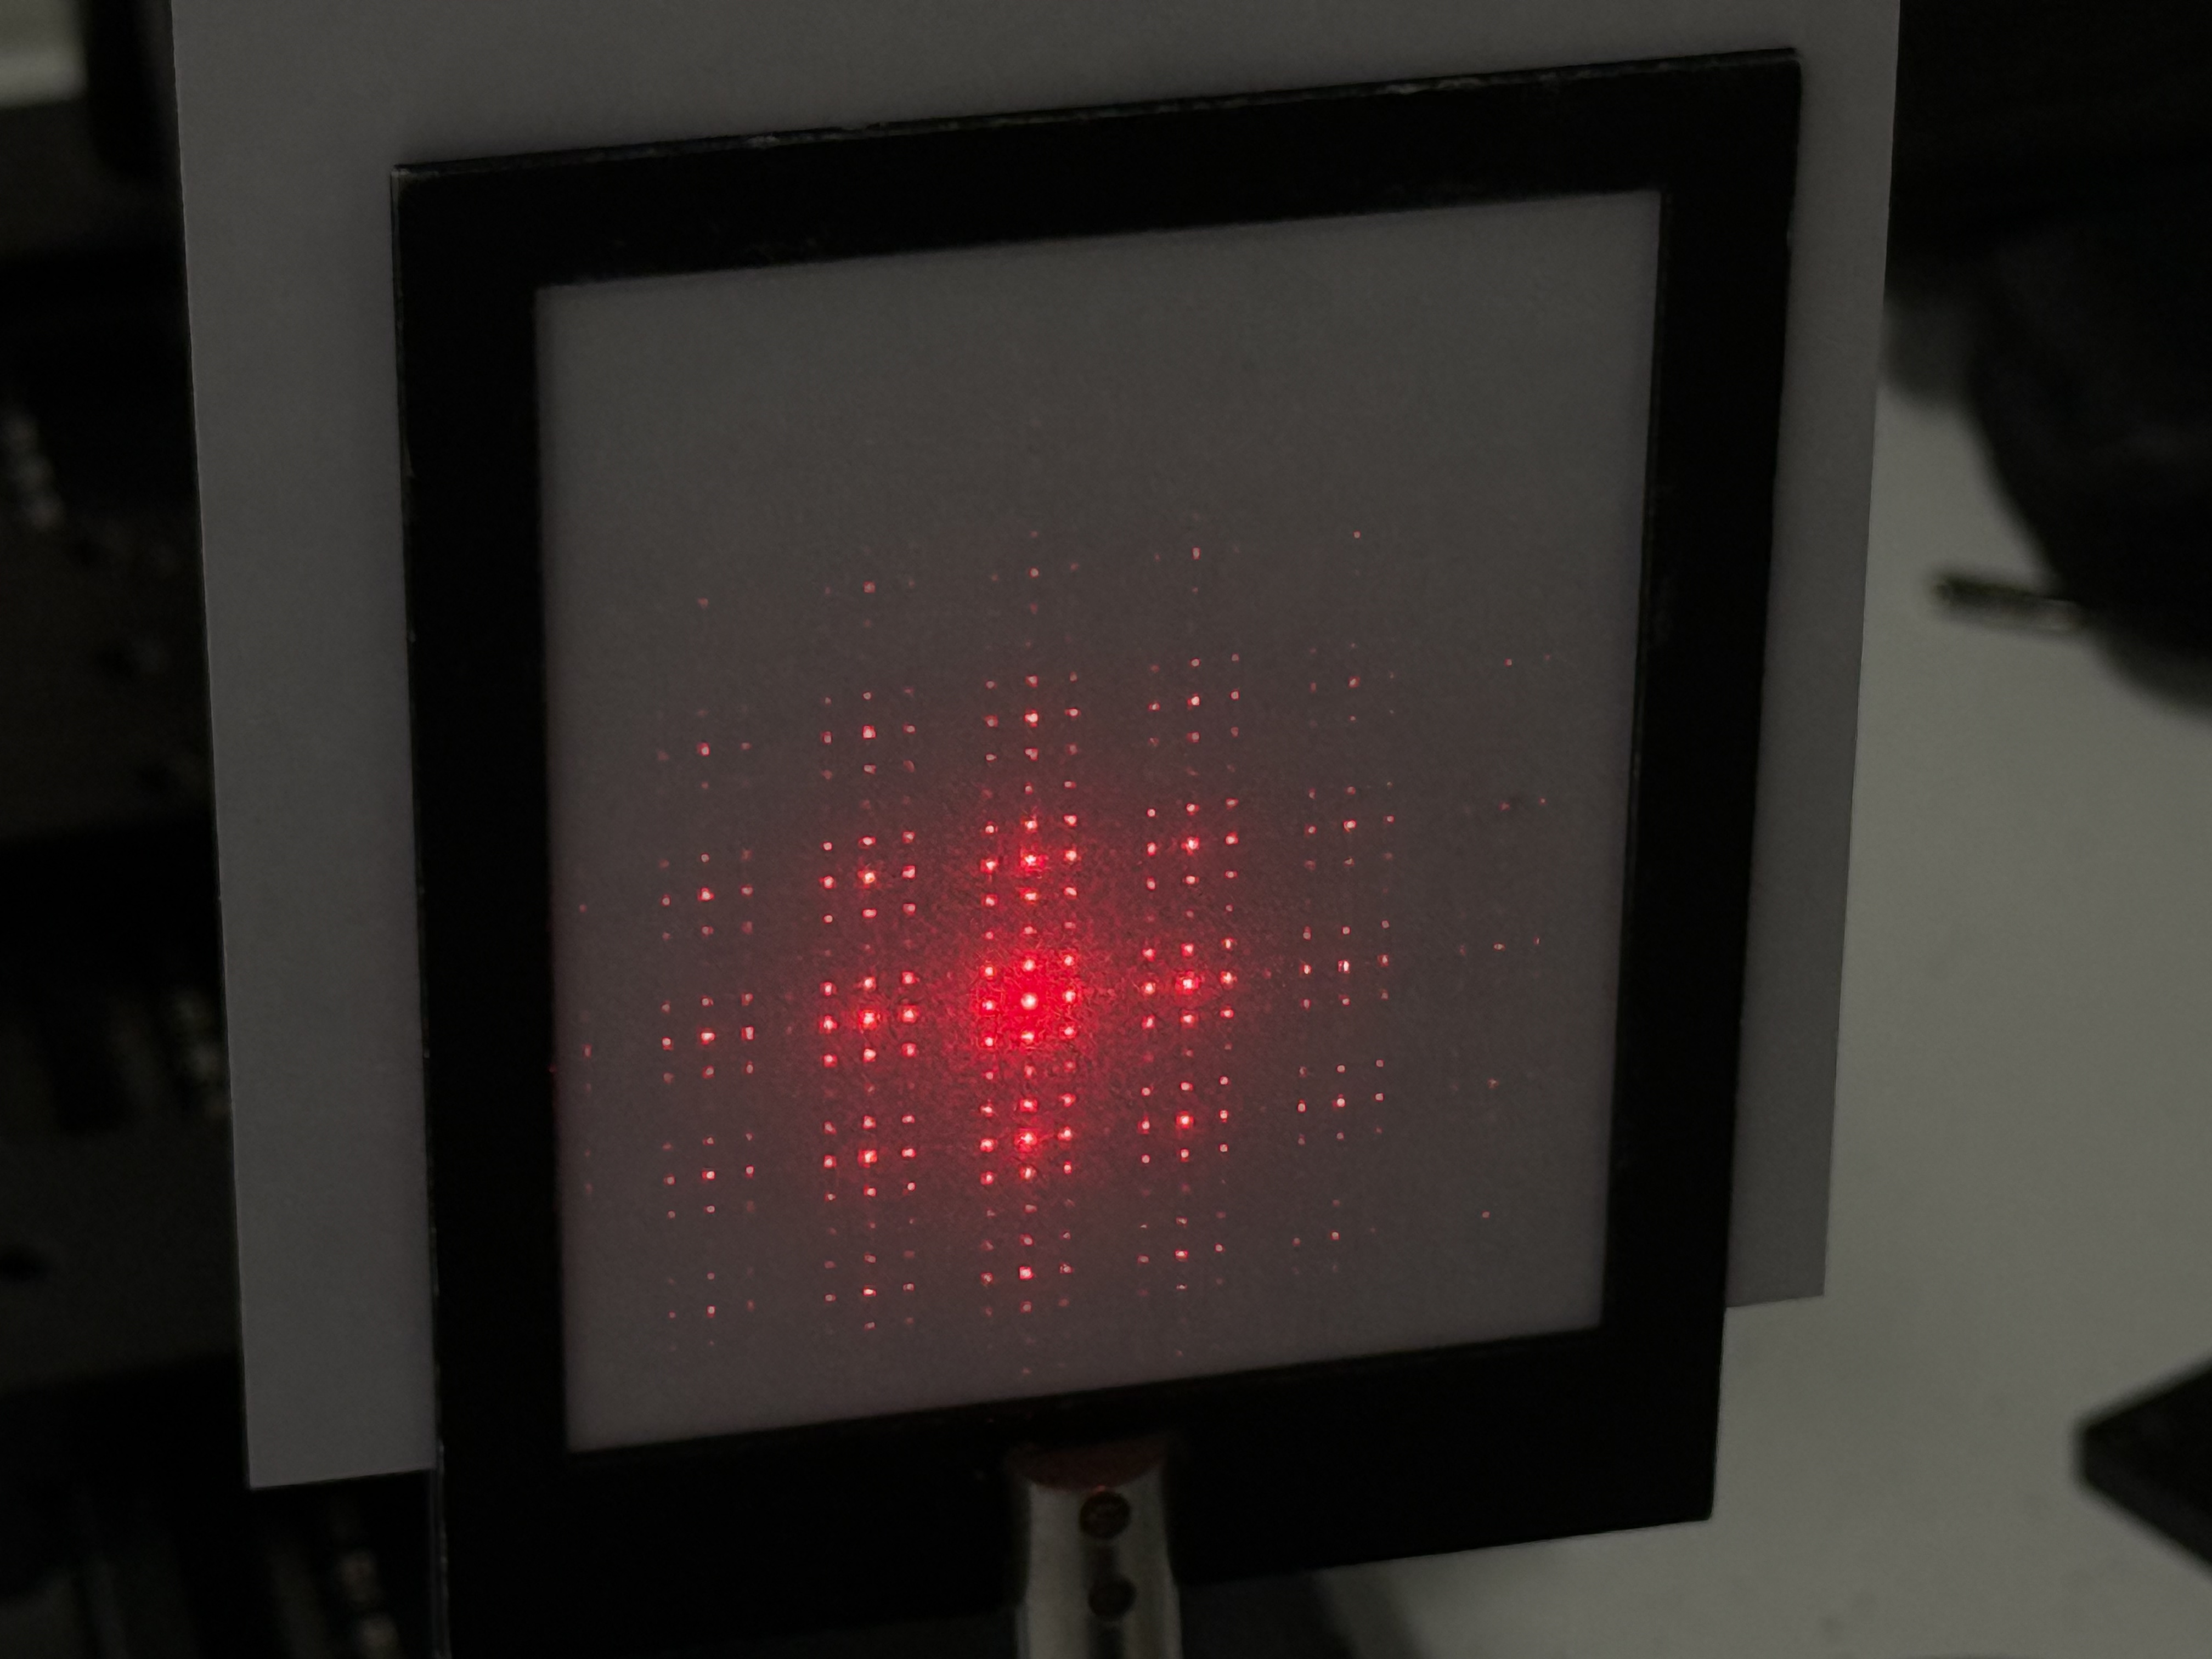
\includegraphics[width=0.9\textwidth]{Data/003-pattern/conv_344_164.png}
        \subcaption{$+0^\circ$}
        \label{fig:convolution_rot_02_00deg}
    \end{subfigure}%
    \hspace{0.03\textwidth}% --- 固定的水平间距 ---
    \begin{subfigure}[b]{0.3\textwidth}
        \centering
        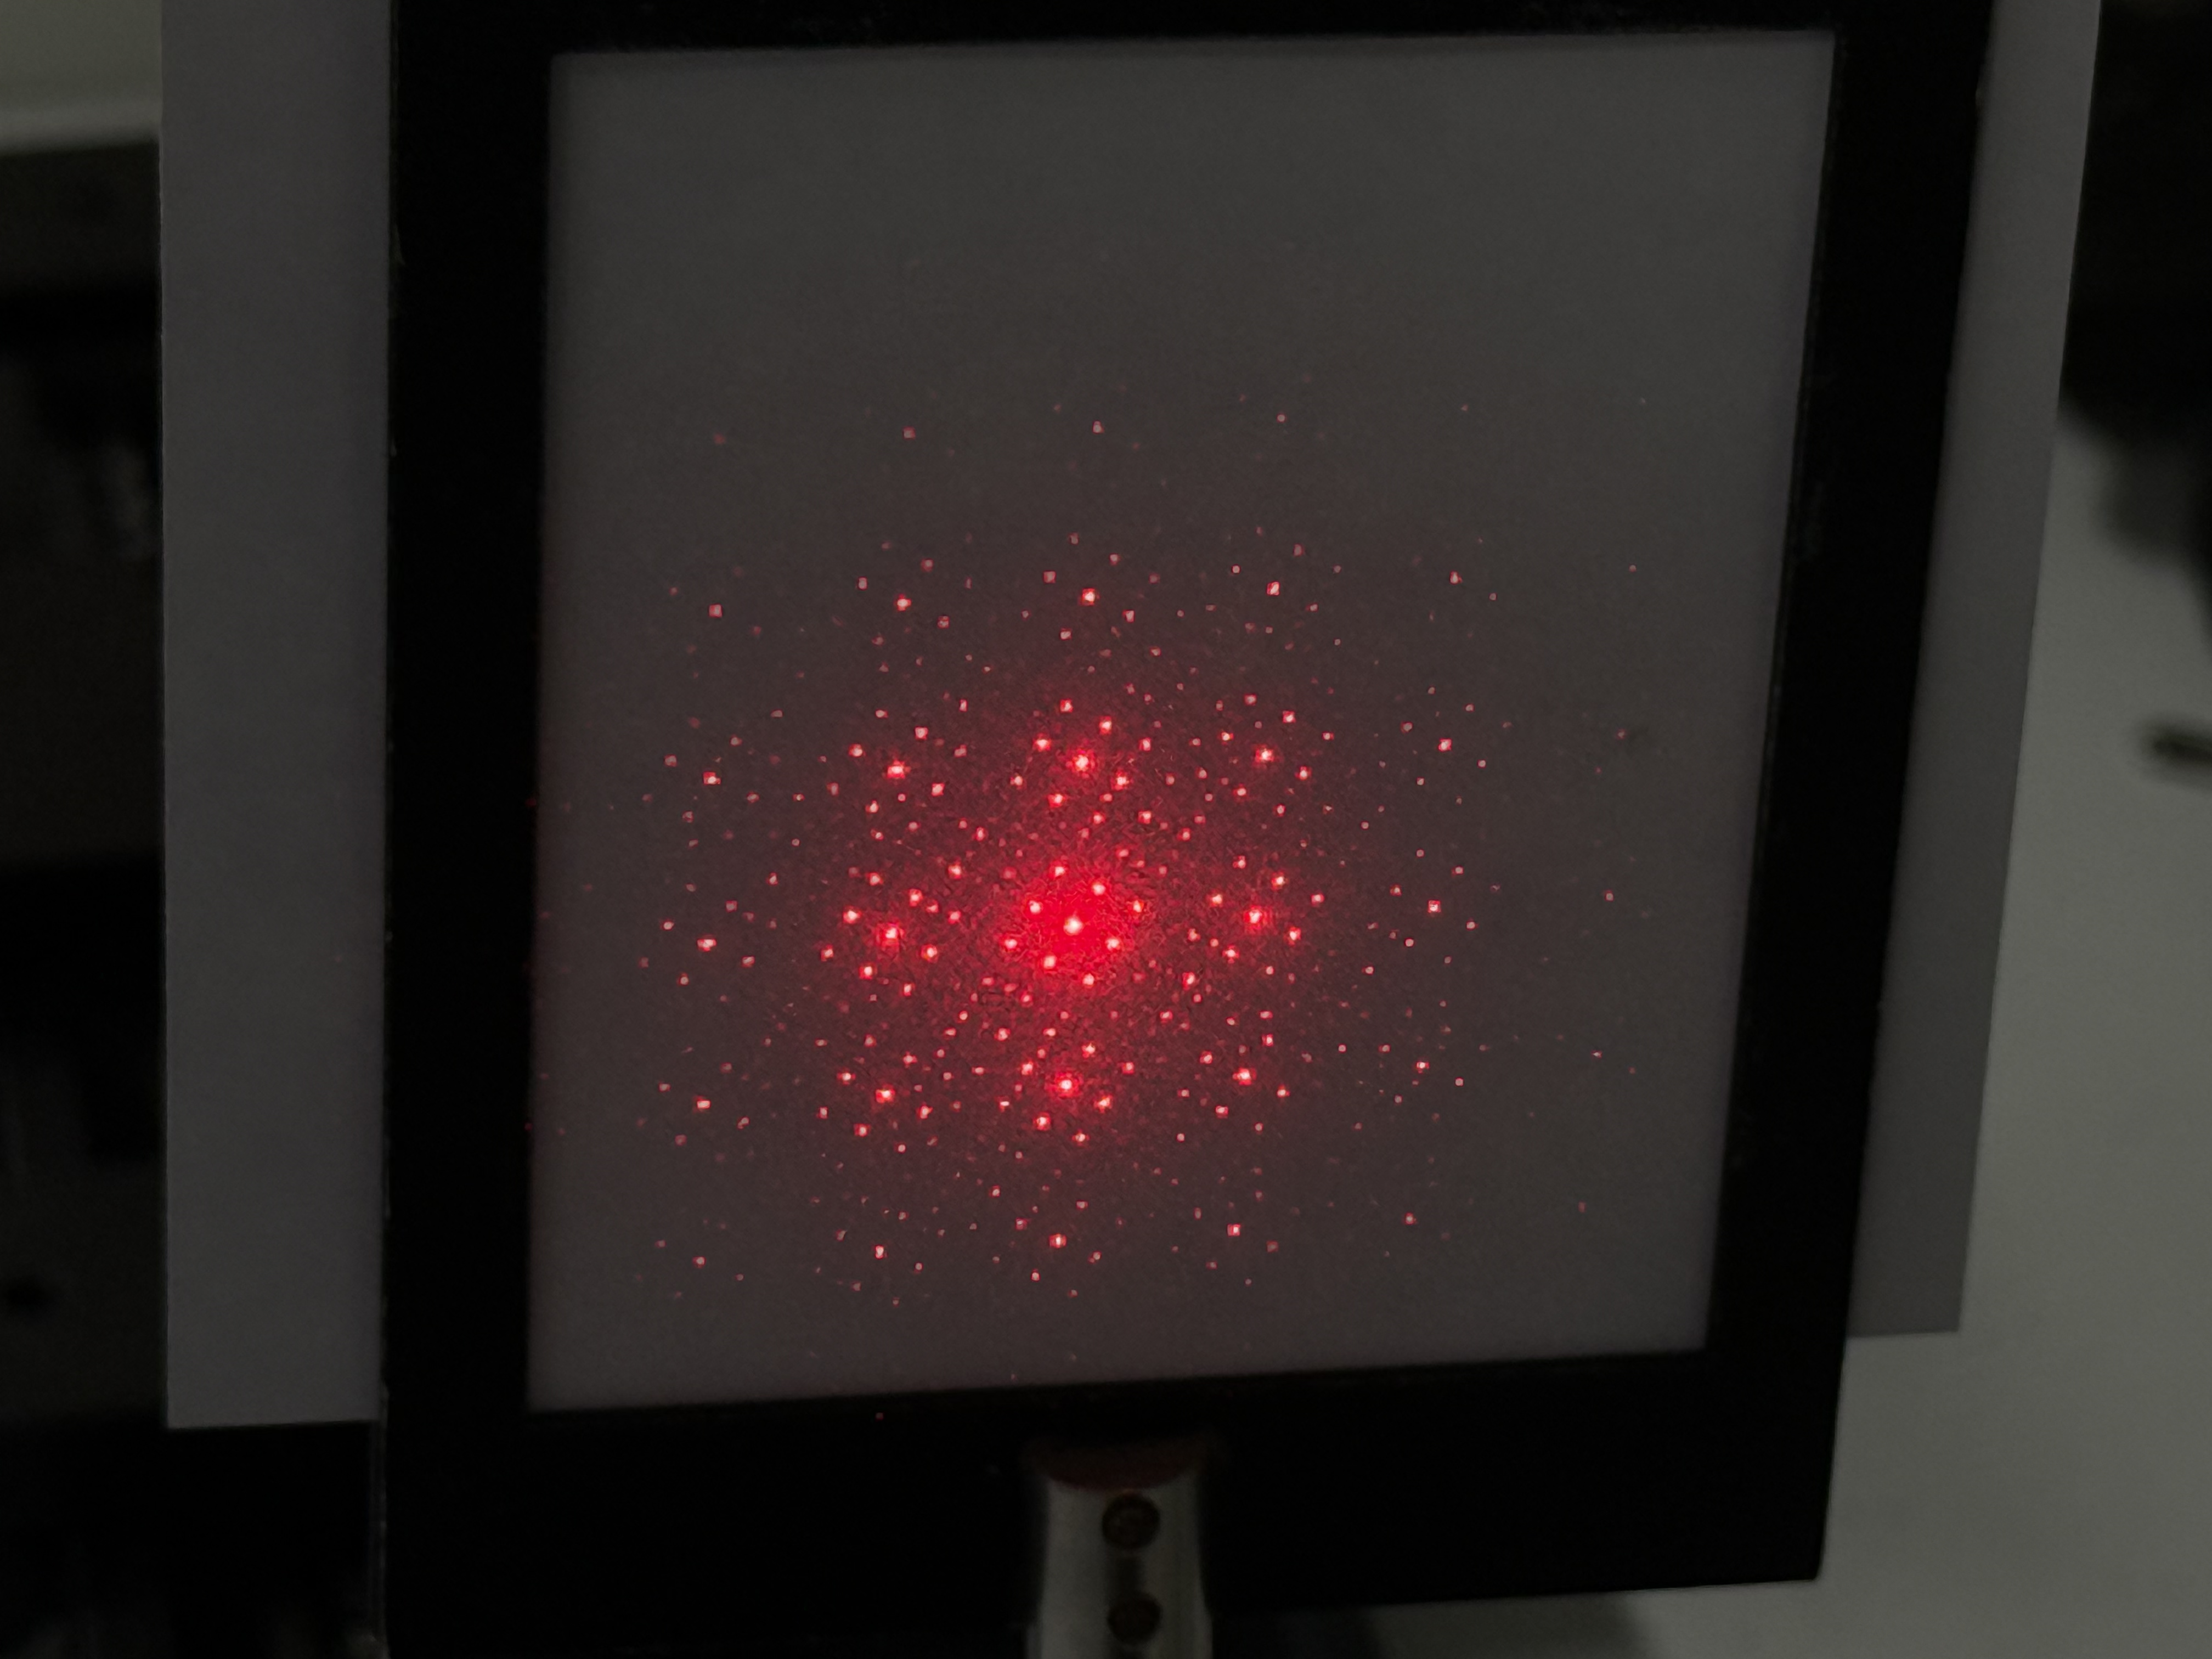
\includegraphics[width=0.9\textwidth]{Data/003-pattern/conv_344_194.png}
        \subcaption{$+30^\circ$}
        \label{fig:convolution_rot_02_30deg}
    \end{subfigure}%
    \hspace{0.03\textwidth}% --- 固定的水平间距 ---
    \begin{subfigure}[b]{0.3\textwidth}
        \centering
        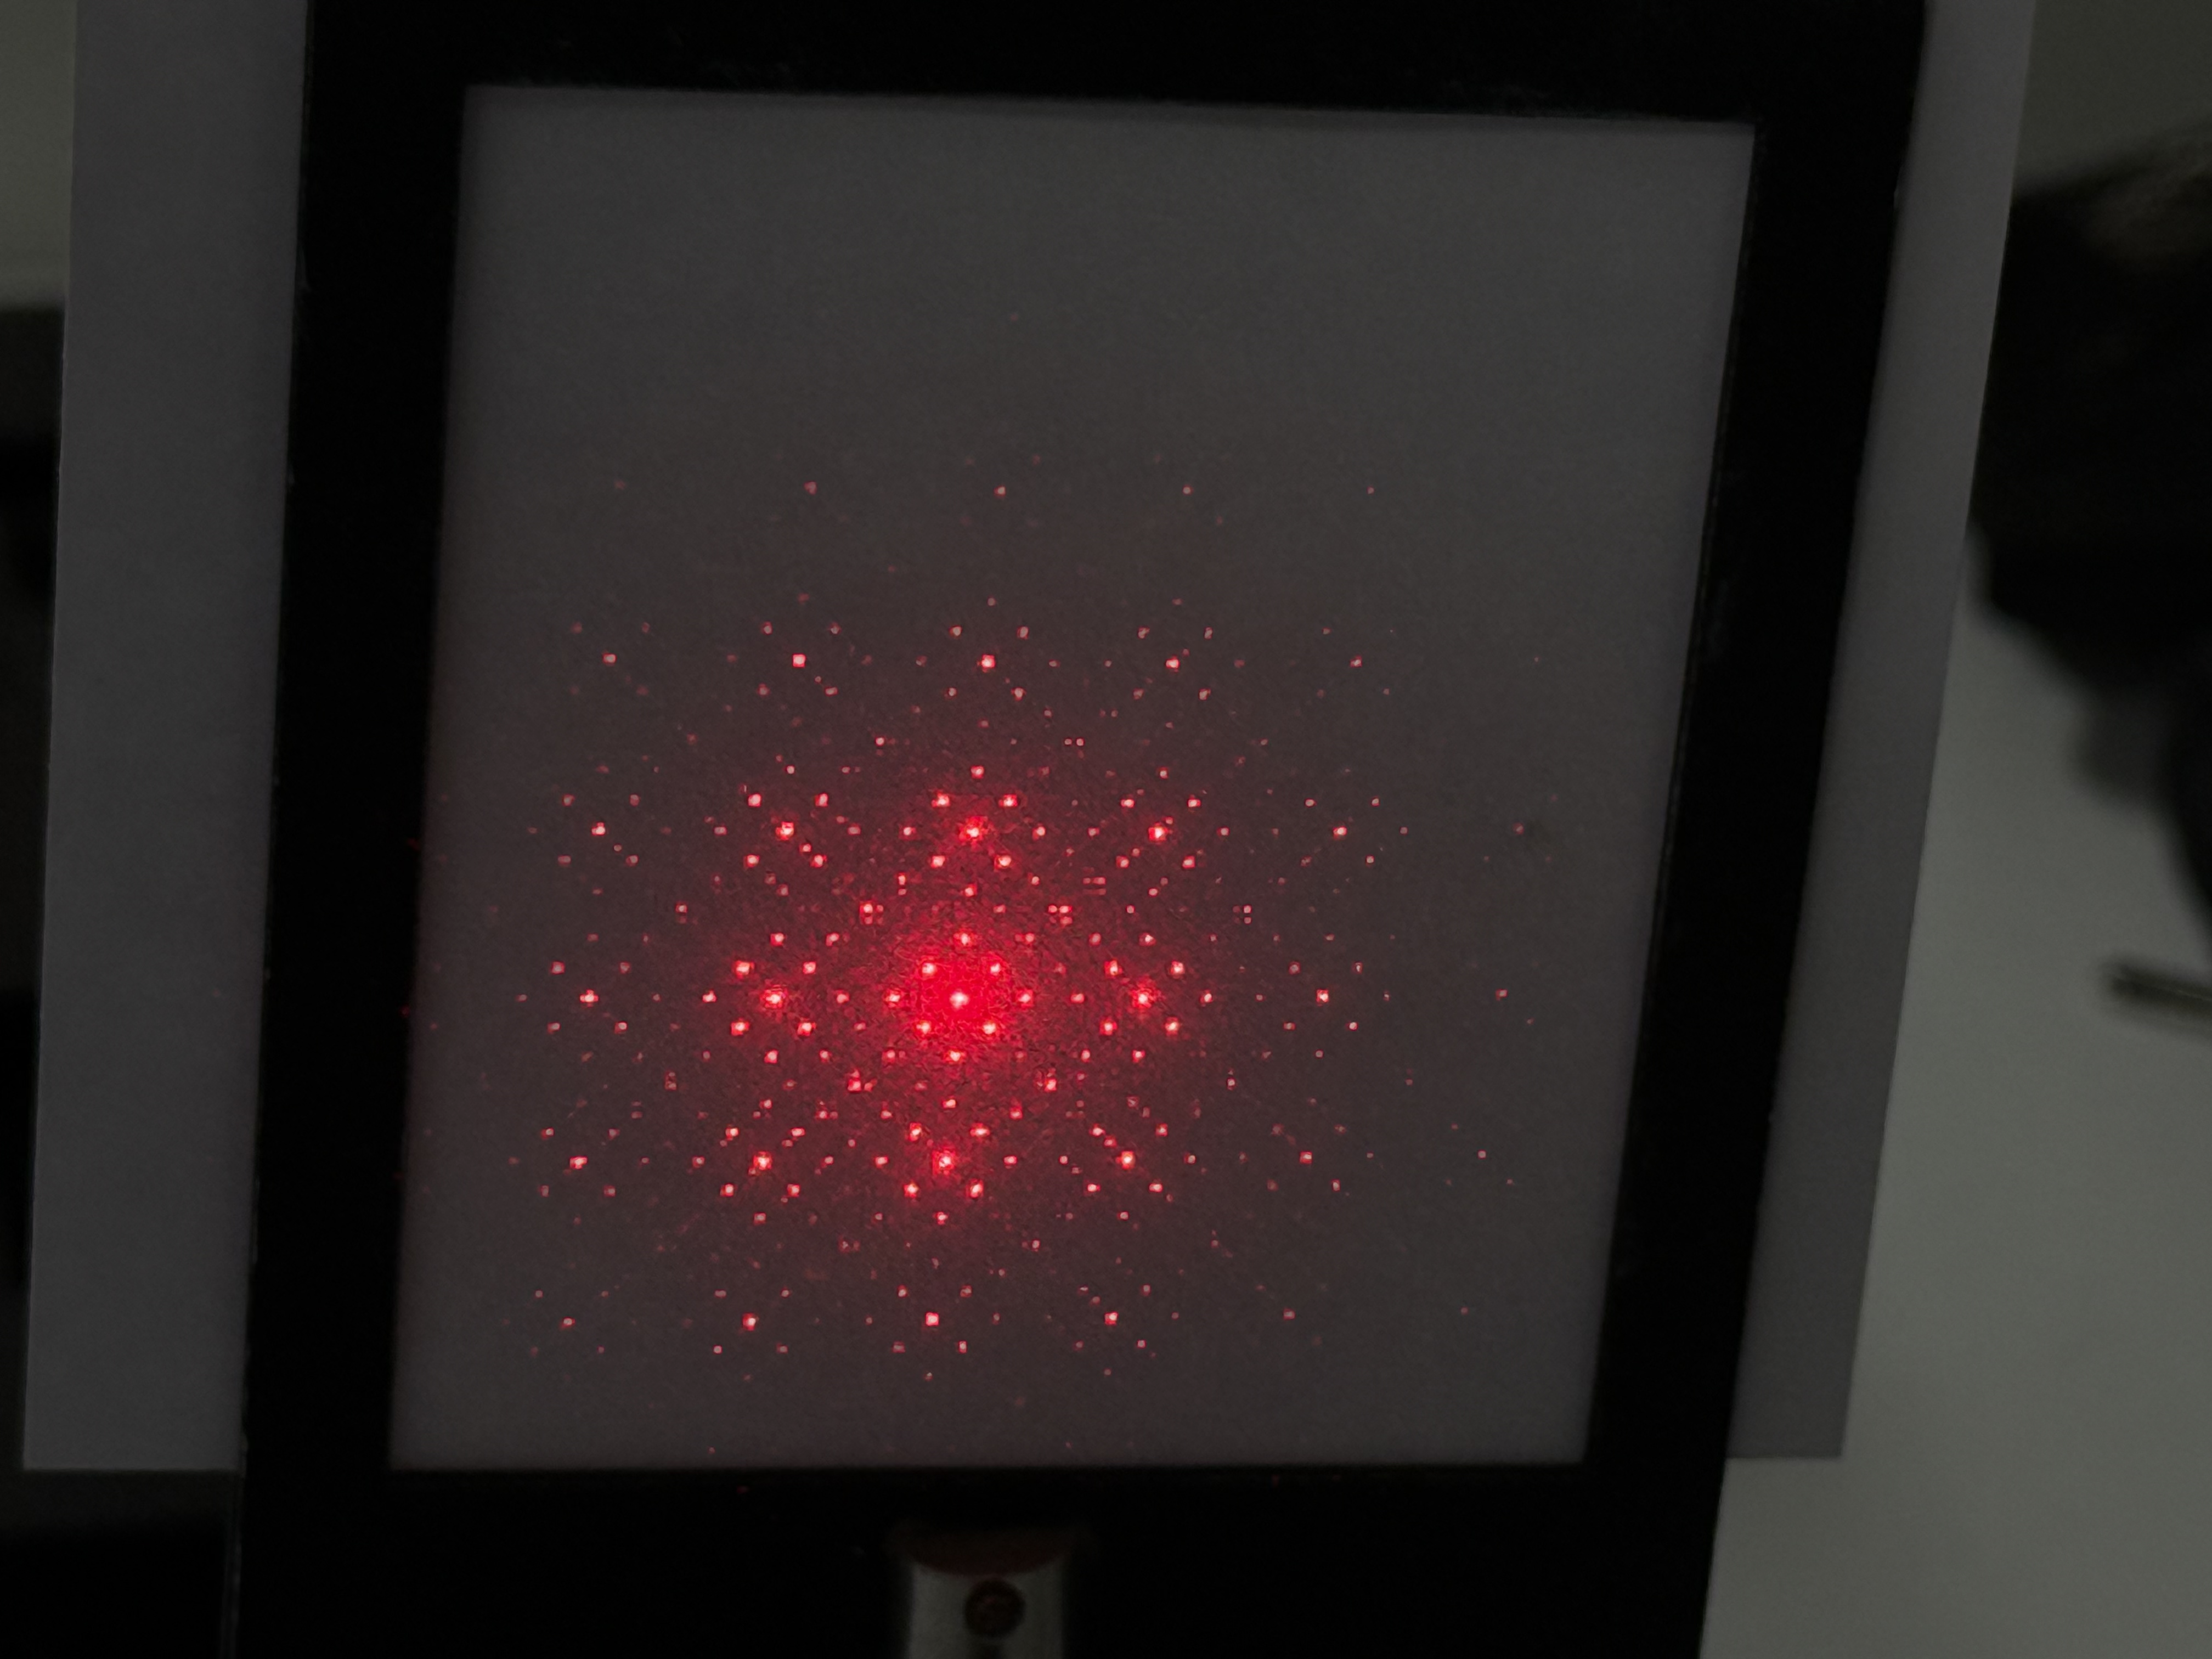
\includegraphics[width=0.9\textwidth]{Data/003-pattern/conv_344_209.png}
        \subcaption{$+45^\circ$}
        \label{fig:convolution_rot_02_45deg}
    \end{subfigure}

    % --- 换行并添加垂直间距 ---

    % --- 第二排:2张图 ---
    % 由于外层有 \centering,这两张图会自动整体居中
    \begin{subfigure}[b]{0.3\textwidth}
        \centering
        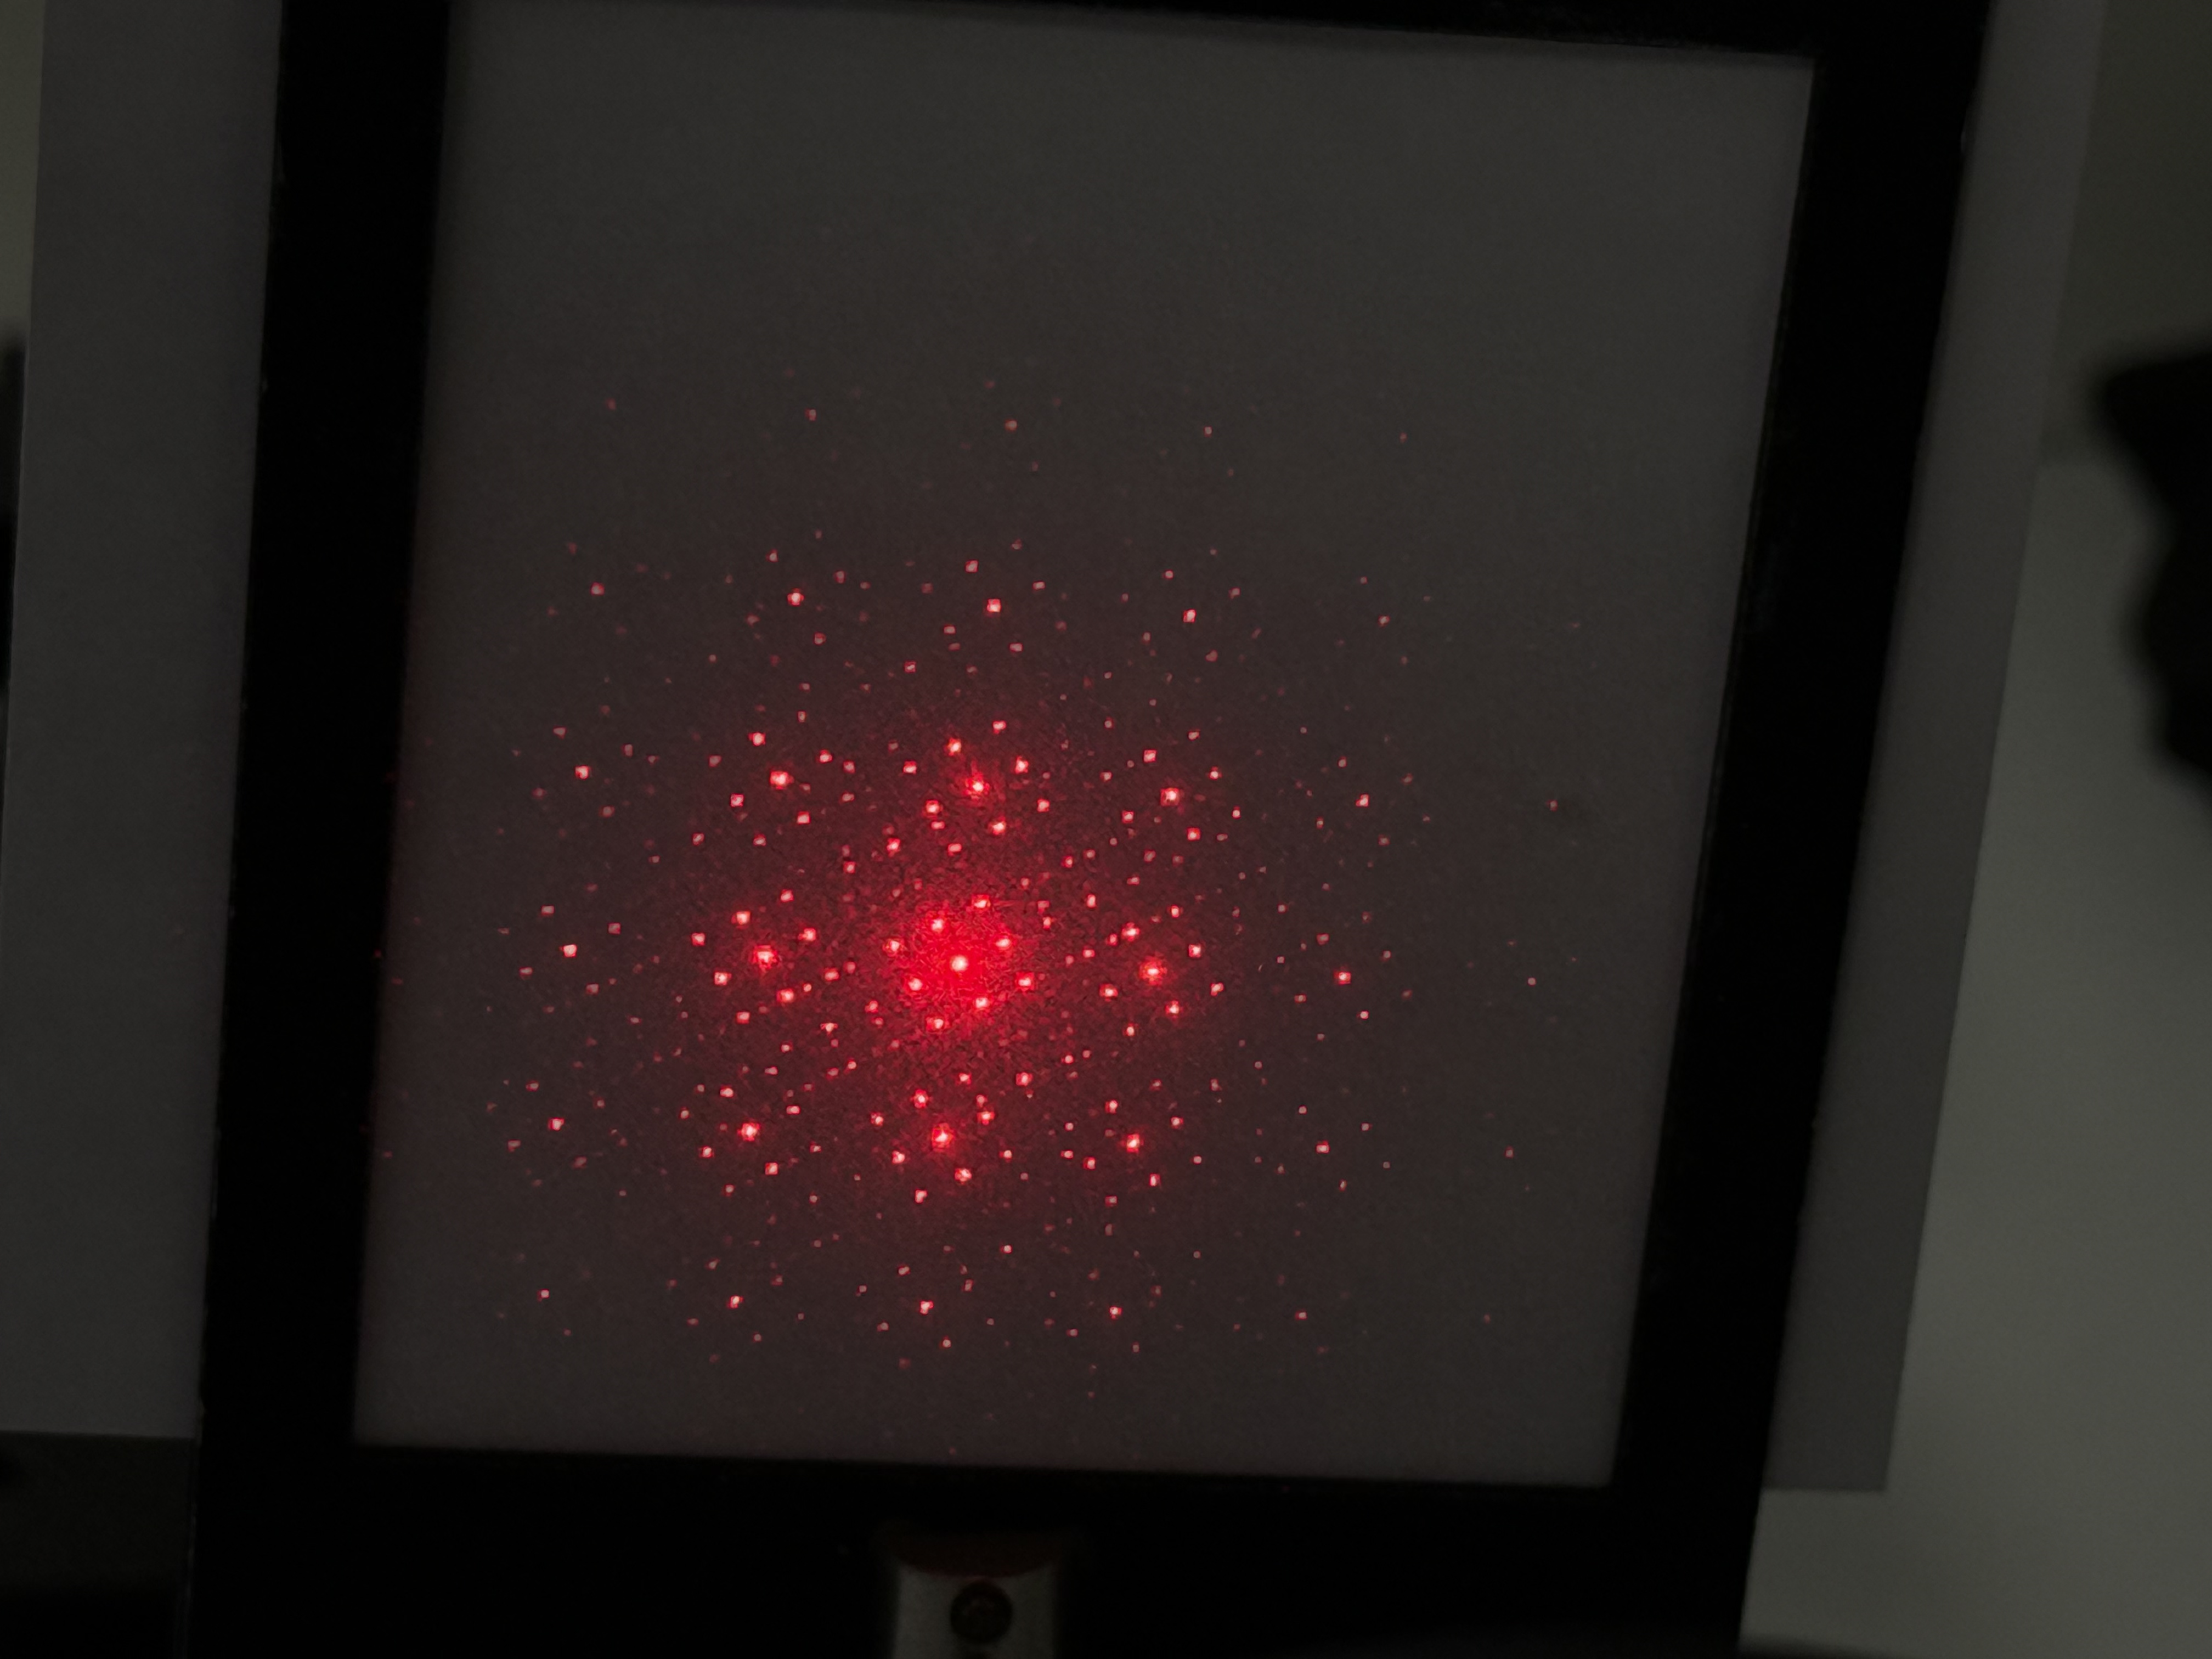
\includegraphics[width=0.9\textwidth]{Data/003-pattern/conv_344_224.png}
        \subcaption{$+60^\circ$}
        \label{fig:convolution_rot_02_60deg}
    \end{subfigure}%
    \hspace{0.03\textwidth}% --- 必须与第一排间距完全一致 ---
    \begin{subfigure}[b]{0.3\textwidth}
        \centering
        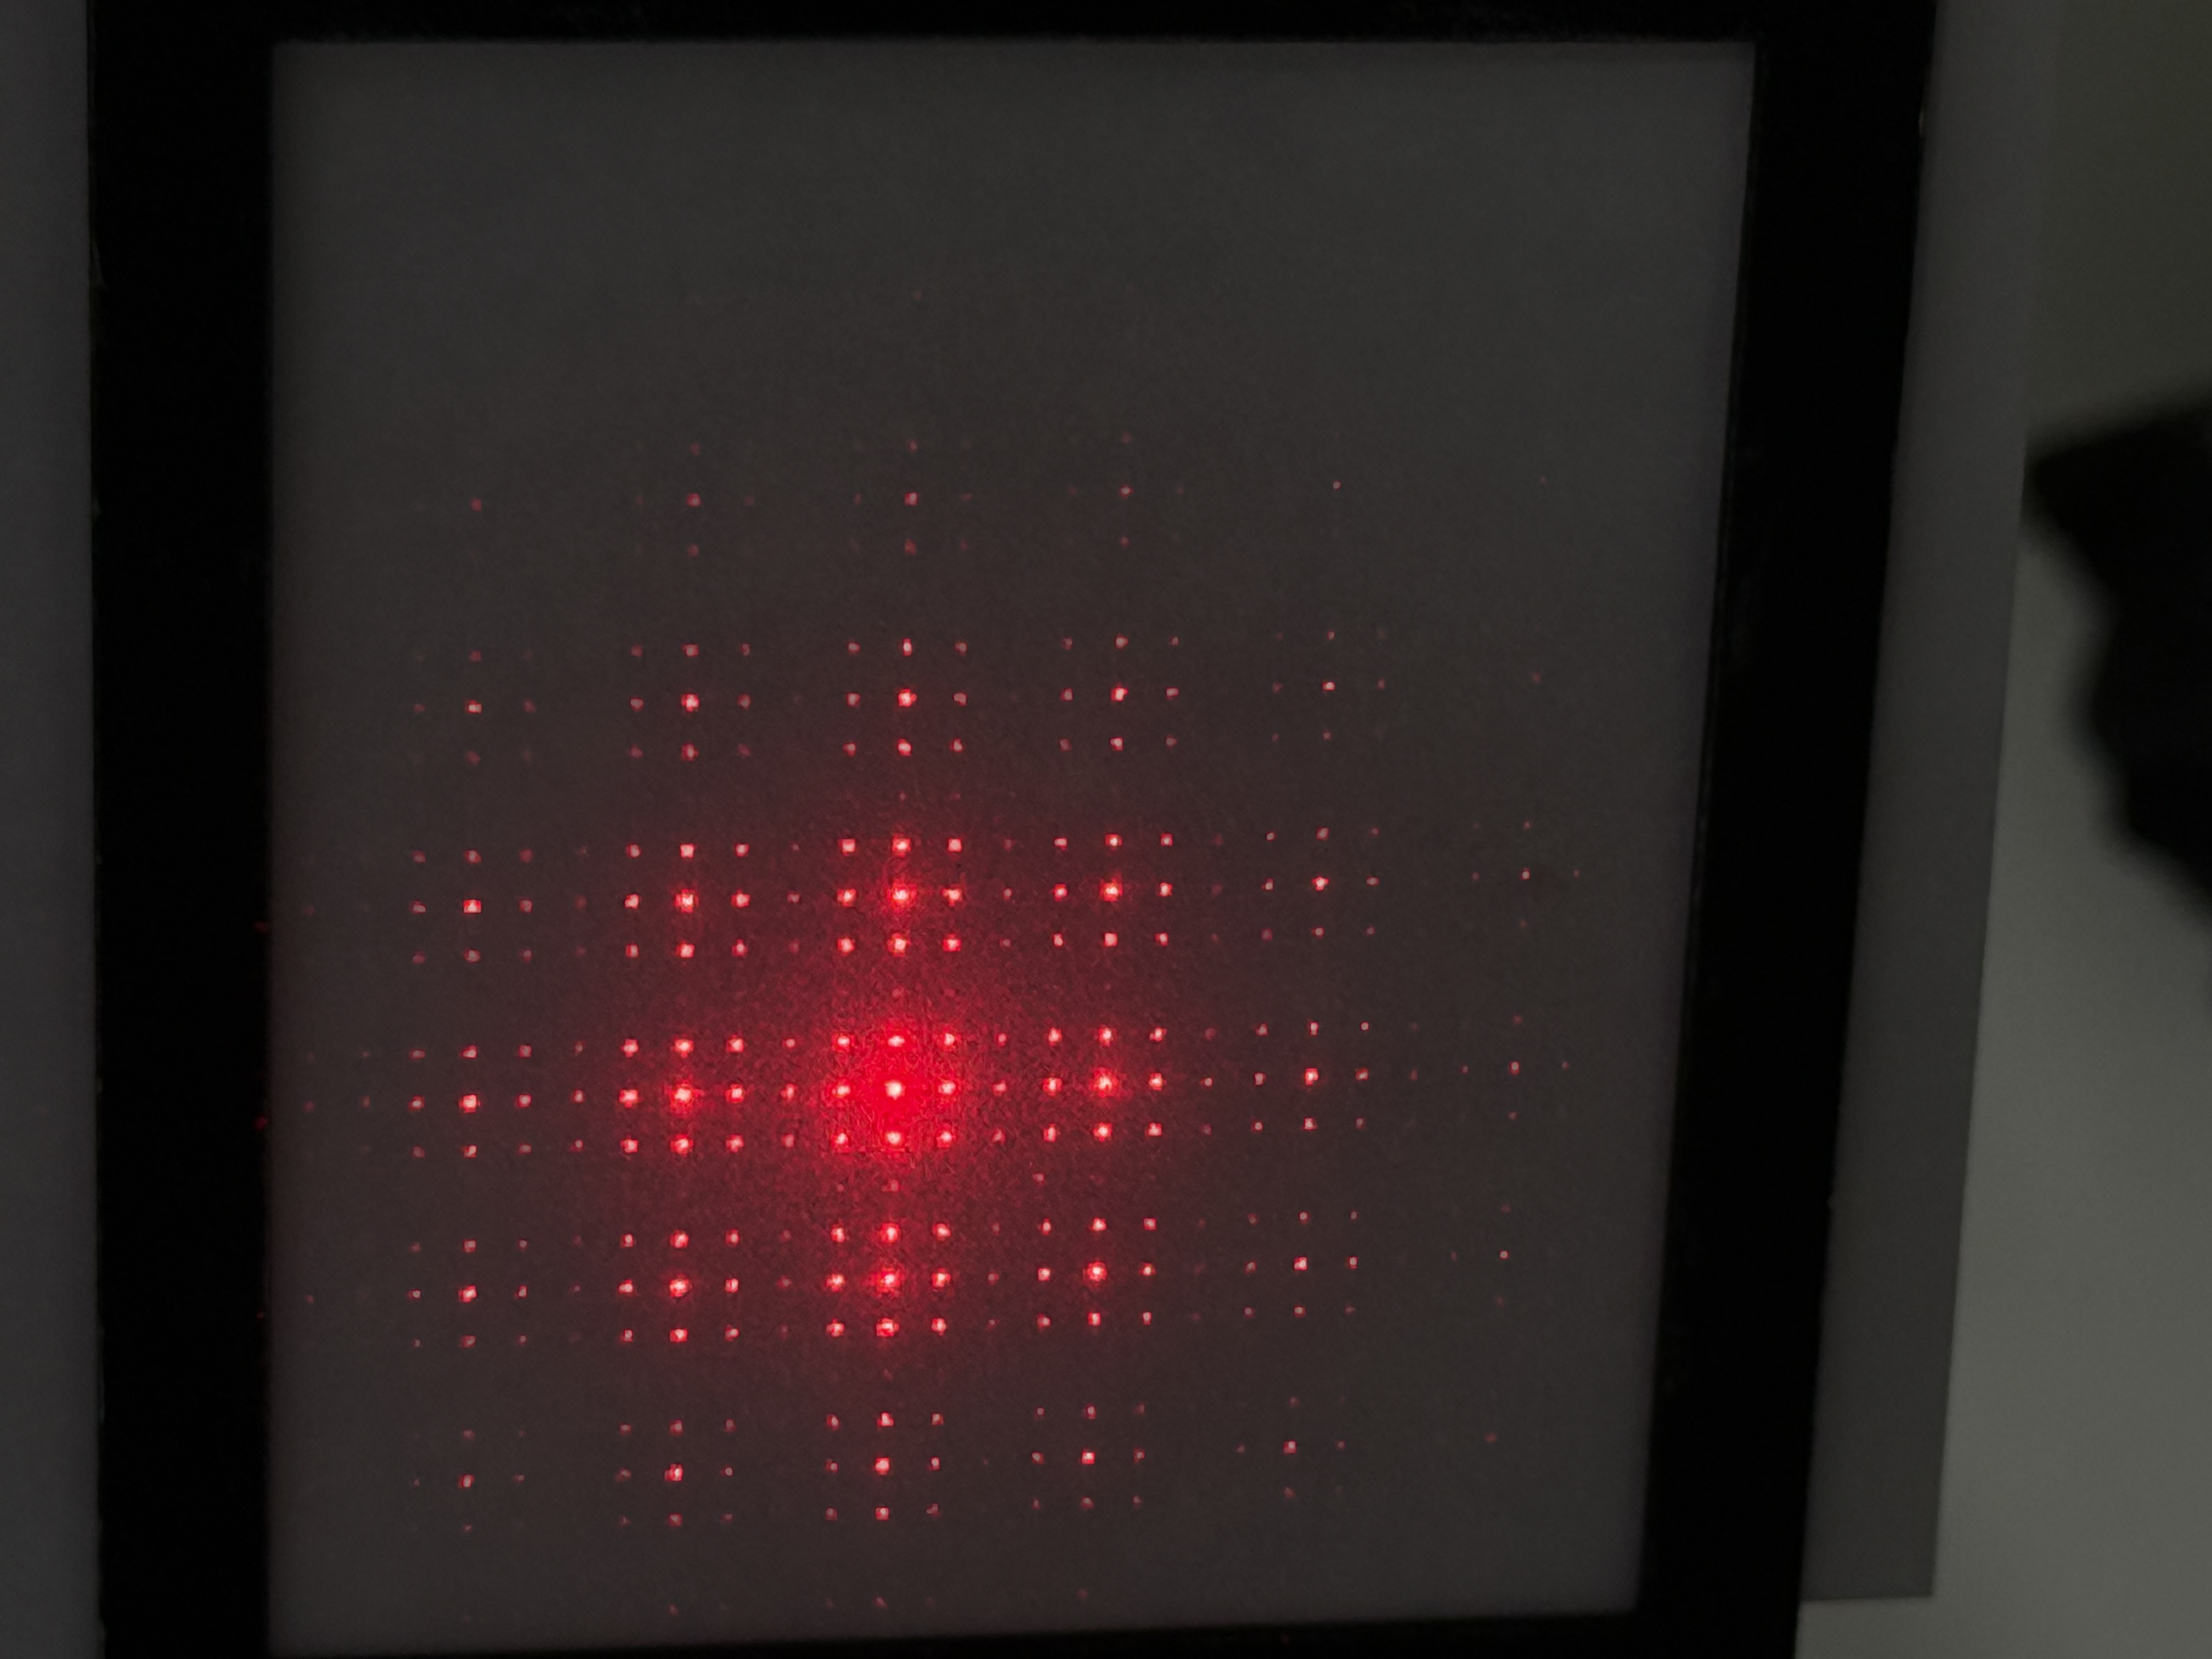
\includegraphics[width=0.9\textwidth]{Data/003-pattern/conv_344_254.png}
        \subcaption{$+90^\circ$}
        \label{fig:convolution_rot_02_90deg}
    \end{subfigure}
    \caption{单独旋转卷积件2至不同角度所得衍射图样}
    \captionnamefont{\wuhao\bf\heiti}
    \captiontitlefont{\wuhao\bf\heiti}
    \label{fig:convolution_rot_02}
\end{figure*}

先后单独旋转卷积件2至一系列不同角度,可观察到:与卷积件2相关联的小周期衍射图样整体形貌不变,取向伴随其旋转而变化;与卷积件1相关联的这些小周期图样的排布取向以及空间周期均无显著变化。

经观察,注意到以下特性:

\begin{enumerate}
    \item 卷积件1,2各自旋转$90^\circ$,对应的衍射图样不变,提示卷积件1,2各自具有$C_4$旋转对称性;
    \item 图\ref{fig:convolution_rot_01_60deg}与图\ref{fig:convolution_rot_02_30deg},图\ref{fig:convolution_rot_01_45deg}与\ref{fig:convolution_rot_02_45deg},图\ref{fig:convolution_rot_01_30deg}与图\ref{fig:convolution_rot_02_60deg}三组图像中,卷积件1,2旋转角度互为补角$90^\circ$,对应的衍射图样相似,提示整体衍射图样仅与卷积件1,2的相对取向有关。
\end{enumerate}

% 卷积件1, 2依次同步转过0, 30, 45, 60, 90度,五张图“上三下二”排布

\subsection{光学微分}


\subsection{\texorpdfstring{$\theta$}{theta} 调制}

%%%%%%%%%%%%%%%%%%%%%%%%%%%%%%%%%%%%%%%%%%%%%%%%%%%%%%%%%%%%%%%%
%  参考文献
%%%%%%%%%%%%%%%%%%%%%%%%%%%%%%%%%%%%%%%%%%%%%%%%%%%%%%%%%%%%%%%%
%  参考文献按GB/T 7714-2015《文后参考文献著录规则》的要求著录. 
%  参考文献在正文中的引用方法:\cite{bib文件条目的第一行}

\renewcommand\refname{\heiti\wuhao\centerline{参考文献}\global\def\refname{参考文献}}
\vskip 12pt


\let\OLDthebibliography\thebibliography
\renewcommand\thebibliography[1]{
  \OLDthebibliography{#1}
  \setlength{\parskip}{0pt}
  \setlength{\itemsep}{0pt plus 0.3ex}
}

{
\renewcommand{\baselinestretch}{0.9}
\liuhao
\bibliographystyle{gbt7714-numerical}
\bibliography{./Report/report}
}

\appendix

\section{部分实验原理推导}

\section{部分实验数据}

\begin{table}[H]
    \centering
    \captionnamefont{\wuhao\bf\heiti}
    \captiontitlefont{\wuhao\bf\heiti}
    \caption{空间成分滤波(一维光栅)实验数据记录} \label{tab:data_1d_filter}
    \liuhao
    \begin{tabular}{c p{5cm} p{5cm}}
        \toprule
        滤波情况(通过的衍射级) & 像面图像特征(定性描述) & 备注(条纹周期等) \\
        \midrule
        0, $\pm 1$ 级 & 条纹清晰,边缘较模糊 & 周期 $d \approx 1/f_0$ \\
        0, $\pm 2$ 级 & 条纹清晰,边缘较模糊 & 周期 $d' \approx 1/(2f_0)$ \\
        0, $\pm 1$, $\pm 2$ 级 & 条纹清晰,边缘较锐利 & 周期 $d \approx 1/f_0$ \\
        仅 0 级 & 均匀亮背景,无条纹 & / \\
        $\pm 1$ 级(滤除 0 级) & 条纹清晰,背景暗,对比度反转 & 周期 $d' \approx 1/(2f_0)$ \\
        全部通过 & 条纹清晰,边缘锐利,接近方波 & 周期 $d \approx 1/f_0$ \\ 
        \bottomrule
    \end{tabular}
\end{table}

\begin{table}[H]
    \centering
    \captionnamefont{\wuhao\bf\heiti}
    \captiontitlefont{\wuhao\bf\heiti}
    \caption{方向滤波(“光”字屏)实验数据记录} \label{tab:data_2d_filter}
    \liuhao
    \begin{tabular}{c p{5cm} p{5cm}}
        \toprule
        滤波器类型 & 像面图像特征(定性描述) & 分析 \\
        \midrule
        无滤波器 & 清晰的“光”字 & 包含所有频率成分 \\
        竖直狭缝(过 0 级) & 仅显示“光”字的竖直笔画 & 滤除了竖直方向的频谱(对应水平笔画) \\
        水平狭缝(过 0 级) & 仅显示“光”字的水平笔画 & 滤除了水平方向的频谱(对应竖直笔画) \\
        45$^\circ$ 狭缝(过 0 级) & 未观察到清晰的特定方向笔画 & “光”字屏主要由水平和竖直结构构成 \\
        \bottomrule
    \end{tabular}
\end{table}


\end{document}